% Supplementary information of the psmc-rs manuscript. Build with `make`
% (Makefile): numbers.tex and tableS1.tex come from make_numbers.py, and
% sn1.tex from experiment/Supplementary_Note_1_Reproducibility.md.
\documentclass[11pt]{article}
\usepackage[a4paper,margin=2.5cm]{geometry}
\usepackage{amsmath}
\usepackage{fontspec}
\setmainfont{texgyretermes}[Extension=.otf,UprightFont=*-regular,BoldFont=*-bold,ItalicFont=*-italic,BoldItalicFont=*-bolditalic]
\usepackage{unicode-math}
\setmathfont{texgyretermes-math.otf}
\usepackage{graphicx}
\usepackage{booktabs}
\usepackage{longtable}
\usepackage{array}
\usepackage{calc}
\usepackage{xcolor}
\usepackage[round]{natbib}
\usepackage{microtype}
\usepackage{caption}
\usepackage[hidelinks]{hyperref}
\usepackage{xurl}
\captionsetup{font=small,labelfont=bf,labelsep=period}
\graphicspath{{../experiment/runs/}}
\setlength{\bibsep}{2pt}
\setlength{\emergencystretch}{1.5em}
\setcounter{secnumdepth}{0}
\newcounter{none}  % pandoc's longtables: \def\LTcaptype{none}
\providecommand{\tightlist}{\setlength{\itemsep}{0pt}\setlength{\parskip}{0pt}}
\makeatletter\def\verbatim@font{\scriptsize\ttfamily}\makeatother
\renewcommand{\thefigure}{S\arabic{figure}}
\renewcommand{\thetable}{S\arabic{table}}
% Generated by manuscript/make_numbers.py from experiment/runs/*/tables; do not edit.

\newcommand{\EoneModels}{4}  % config.E1.models
\newcommand{\EoneReps}{10}  % config.E1.replicates
\newcommand{\EoneGenomes}{40}  % models x replicates
\newcommand{\EoneChroms}{10}  % config.E1.genome
\newcommand{\EoneChromMb}{50}  % config.E1.genome
\newcommand{\EoneGenomeMb}{500}  % config.E1.genome
\newcommand{\EoneRsCRmseMin}{\ensuremath{3.7\times10^{-6}}}  % E1_rs_vs_c min rmse
\newcommand{\EoneRsCRmseMax}{\ensuremath{2.0\times10^{-4}}}  % E1_rs_vs_c max rmse
\newcommand{\EoneRsCRmseMedian}{\ensuremath{2.5\times10^{-5}}}  % E1_rs_vs_c median rmse
\newcommand{\EoneRsCMaxAbs}{\ensuremath{6.6\times10^{-4}}}  % E1_rs_vs_c max abs in window
\newcommand{\EoneAnyMax}{\ensuremath{2.0}}  % E1_rs_vs_c max abs any interval
\newcommand{\EoneAnyModel}{expansion}  % E1_rs_vs_c worst any interval
\newcommand{\EoneAnyReplicate}{5}  % E1_rs_vs_c worst any interval
\newcommand{\EoneAnySecond}{\ensuremath{6.6\times10^{-4}}}  % E1_rs_vs_c second largest any interval
\newcommand{\EoneRunawayC}{\ensuremath{1.1\times10^{6}}}  % E1_curves worst replicate, C psmc's first lambda
\newcommand{\EoneRunawayCNe}{\ensuremath{2.5\times10^{9}}}  % E1_curves worst replicate, C psmc's Ne in the first interval
\newcommand{\EoneRunawayKy}{\ensuremath{4.8}}  % E1_curves worst replicate, end of the first free lambda (ky)
\newcommand{\EoneParamRelMax}{\ensuremath{5.5\times10^{-4}}}  % E1_rs_vs_c max |rel diff| theta, rho, t_max
\newcommand{\EoneLoglikeRelMax}{\ensuremath{3.5\times10^{-8}}}  % E1_rs_vs_c loglike_max_rel_diff (any iteration)
\newcommand{\EoneLoglikeLastRelMax}{\ensuremath{1.3\times10^{-8}}}  % E1_replicates loglike_common (the last iteration both report)
\newcommand{\EoneLoglikeFirstRelMax}{\ensuremath{7.0\times10^{-13}}}  % E1_rs_vs_c loglike_iteration0_rel_diff
\newcommand{\EoneConstantTruthC}{\ensuremath{0.048}}  % E1_table1 rmse_truth_c_mean
\newcommand{\EoneConstantTruthRs}{\ensuremath{0.048}}  % E1_table1 rmse_truth_rs_mean
\newcommand{\EoneBottleneckTruthC}{\ensuremath{0.291}}  % E1_table1 rmse_truth_c_mean
\newcommand{\EoneBottleneckTruthRs}{\ensuremath{0.291}}  % E1_table1 rmse_truth_rs_mean
\newcommand{\EoneExpansionTruthC}{\ensuremath{0.240}}  % E1_table1 rmse_truth_c_mean
\newcommand{\EoneExpansionTruthRs}{\ensuremath{0.240}}  % E1_table1 rmse_truth_rs_mean
\newcommand{\EoneZigzagTruthC}{\ensuremath{0.138}}  % E1_table1 rmse_truth_c_mean
\newcommand{\EoneZigzagTruthRs}{\ensuremath{0.138}}  % E1_table1 rmse_truth_rs_mean
\newcommand{\EoneMonotoneRuns}{80}  % E6_S1_summary replicates_monotone
\newcommand{\EoneRuns}{80}  % E6_S1_summary replicates
\newcommand{\EtwoRsCRmseMin}{\ensuremath{9.7\times10^{-6}}}  % E2_rs_vs_c
\newcommand{\EtwoRsCRmseMax}{\ensuremath{2.8\times10^{-4}}}  % E2_rs_vs_c
\newcommand{\EtwoRsCMaxAbs}{\ensuremath{4.5\times10^{-4}}}  % E2_rs_vs_c
\newcommand{\EtwoHumanRmse}{\ensuremath{9.7\times10^{-6}}}  % E2_rs_vs_c NA12878
\newcommand{\EtwoParamRelMax}{\ensuremath{1.0\times10^{-3}}}  % E2_fit_summary theta, rho, t_max
\newcommand{\EtwoLoglikeRelMax}{\ensuremath{2.3\times10^{-7}}}  % E2_fit_summary loglike_common
\newcommand{\EtwoLoglikeFirstRelMax}{\ensuremath{6.9\times10^{-14}}}  % E2_rs_vs_c loglike_iteration0_rel_diff
\newcommand{\EtwoHumanSequences}{22}  % E2_fit_summary NA12878 sequences
\newcommand{\EtwoTurtleSeqMin}{34}  % E2_fit_summary turtle sequences
\newcommand{\EtwoTurtleSeqMax}{1,220}  % E2_fit_summary turtle sequences
\newcommand{\EtwoHumanTrunks}{59}  % E2_bootstrap NA12878 trunks
\newcommand{\EtwoBootReps}{100}  % E2_bootstrap replicates
\newcommand{\EtwoBootIdentical}{all}  % E2_bootstrap main_identical_to_fit
\newcommand{\EtwoBootThreads}{50}  % E2_bootstrap threads
\newcommand{\EtwoBandWidthMin}{\ensuremath{0.07}}  % E2_bootstrap band_width_log10_median
\newcommand{\EtwoBandWidthMax}{\ensuremath{0.15}}  % E2_bootstrap band_width_log10_median
\newcommand{\EtwoPeakMin}{\ensuremath{1.4}}  % E2_split_patterns default recent_max_vs_plateau
\newcommand{\EtwoPeakMax}{\ensuremath{4.6}}  % E2_split_patterns default recent_max_vs_plateau
\newcommand{\EtwoPeaksDefault}{3}  % E2_split_patterns default recent_peak
\newcommand{\EtwoPeaksSplit}{0}  % E2_split_patterns split recent_peak
\newcommand{\EtwoSplitFits}{6}  % E2_split_patterns split rows
\newcommand{\EtwoSplitGainMin}{\ensuremath{49}}  % E2_split_patterns loglike_gain_vs_default
\newcommand{\EtwoSplitGainMax}{\ensuremath{586}}  % E2_split_patterns loglike_gain_vs_default
\newcommand{\EtwoSplitOlderMax}{\ensuremath{1.5\times10^{-2}}}  % E2_split_curves: split vs default after the recent intervals, same times
\newcommand{\EtwoSplitThetaMax}{6.8\%}  % E2_split_patterns theta of split vs default
\newcommand{\EtwoBootPeakEmy}{56}  % E2_bootstrap_replicates recent_peak, E. subglobosa
\newcommand{\EtwoBootPeakHyd}{100}  % E2_bootstrap_replicates recent_peak, H. tectifera
\newcommand{\EtwoBootPeakPel}{100}  % E2_bootstrap_replicates recent_peak, P. castaneus
\newcommand{\EtwoTurtles}{3}  % E2_fit_summary turtle genomes
\newcommand{\EthreeRepeats}{5}  % config.E3.repeats
\newcommand{\EthreeBigMb}{3,000}  % config.E3.genome_sizes_mb
\newcommand{\EthreeBigChroms}{30}  % E3_table2 chromosomes
\newcommand{\EthreeCWall}{4,446}  % E3_table2 c 1 thread
\newcommand{\EthreeCMin}{\ensuremath{74}}  % E3_table2 c 1 thread (min)
\newcommand{\EthreeRsOneWall}{519}  % E3_table2 rs02 1 thread
\newcommand{\EthreeRsZeroWall}{6,193}  % E3_table2 rs01 1 thread
\newcommand{\EthreeSpeedOne}{\ensuremath{8.6}}  % E3_table2 rs02 1 speedup
\newcommand{\EthreeRsWallOne}{\ensuremath{519}}  % E3_table2 rs02 1 wall
\newcommand{\EthreeSpeedEight}{\ensuremath{63}}  % E3_table2 rs02 8 speedup
\newcommand{\EthreeRsWallEight}{\ensuremath{70.6}}  % E3_table2 rs02 8 wall
\newcommand{\EthreeSpeedSixteen}{\ensuremath{123}}  % E3_table2 rs02 16 speedup
\newcommand{\EthreeRsWallSixteen}{\ensuremath{36.0}}  % E3_table2 rs02 16 wall
\newcommand{\EthreeSpeedThirty}{\ensuremath{243}}  % E3_table2 rs02 30 speedup
\newcommand{\EthreeRsWallThirty}{\ensuremath{18.3}}  % E3_table2 rs02 30 wall
\newcommand{\EthreeRsZeroSpeedThirty}{\ensuremath{14}}  % E3_table2 rs01 30 speedup
\newcommand{\EthreeRsZeroRel}{\ensuremath{0.72}}  % E3_table2 rs01 1 speedup
\newcommand{\EthreeCMem}{1,062}  % E3_table2 c peak MB
\newcommand{\EthreeRsMemOne}{\ensuremath{36}}  % E3_table2 rs02 1 peak MB
\newcommand{\EthreeRsMemThirty}{\ensuremath{148}}  % E3_table2 rs02 30 peak MB
\newcommand{\EthreeRsZeroMemThirty}{14,959}  % E3_table2 rs01 30 peak MB
\newcommand{\EthreeRsZeroMemOne}{2,511}  % E3_table2 rs01 1 peak MB
\newcommand{\EthreeSpeedOneMin}{\ensuremath{8.5}}  % E3_table2 rs02 1 thread speedup, every size
\newcommand{\EthreeSpeedOneMax}{\ensuremath{8.8}}  % E3_table2 rs02 1 thread speedup, every size
\newcommand{\EthreeChromWall}{\ensuremath{17.3}}  % E3_table2 rs02 one 100 Mb chromosome, 1 thread
\newcommand{\EthreeChromWallMin}{\ensuremath{17.24}}  % E3_table2 rs02 100 Mb, any threads
\newcommand{\EthreeChromWallMax}{\ensuremath{17.25}}  % E3_table2 rs02 100 Mb, any threads
\newcommand{\EthreeRoundMin}{\ensuremath{17.2}}  % E3_table2 rs02 wall / ceil(chromosomes / threads)
\newcommand{\EthreeRoundMax}{\ensuremath{18.3}}  % E3_table2 rs02 wall / ceil(chromosomes / threads)
\newcommand{\EthreeEffMin}{\ensuremath{0.90}}  % E3_thread_scaling efficiency
\newcommand{\EthreeEffMax}{\ensuremath{0.99}}  % E3_thread_scaling efficiency
\newcommand{\EthreeEffCap}{\ensuremath{0.94}}  % whole chromosomes per thread: min over t of n / (t ceil(n / t))
\newcommand{\EthreeRuns}{155}  % E3_runs rows
\newcommand{\EthreeCleanRuns}{155}  % E3_runs clean
\newcommand{\EthreeNodes}{5}  % E3_runs hostname
\newcommand{\EthreeSpreadMaxMost}{3.5\%}  % E3_table2 (max-min)/median, second largest
\newcommand{\EthreeDetRsIdentical}{75}  % E3_determinism rs02
\newcommand{\EthreeDetRsTotal}{75}  % E3_determinism rs02
\newcommand{\EthreeDetCIdentical}{20}  % E3_determinism c
\newcommand{\EthreeDetCTotal}{20}  % E3_determinism c
\newcommand{\EthreeDetRsZeroIdentical}{30}  % E3_determinism rs01
\newcommand{\EthreeDetRsZeroTotal}{60}  % E3_determinism rs01
\newcommand{\EthreeRsZeroDiffMax}{\ensuremath{2.5\times10^{-5}}}  % E3_determinism rs01 max_rel_diff_params
\newcommand{\EthreeCpu}{AMD EPYC 7702}  % E3_environment machine.cpu
\newcommand{\EthreeCores}{128}  % E3_environment machine.cpu_count
\newcommand{\EfourDispThirtyFqTheta}{34.9\%}  % E4_routes dispersed30 fq2psmcfa -theta_rel (median)
\newcommand{\EfourDispThirtyFqRmse}{\ensuremath{0.36}}  % E4_routes dispersed30 fq2psmcfa rmse vs complete
\newcommand{\EfourDispThirtyAutoTheta}{1.8\%}  % E4_routes dispersed30 mask_auto -theta_rel (median)
\newcommand{\EfourDispThirtyAutoRmse}{\ensuremath{0.07}}  % E4_routes dispersed30 mask_auto rmse vs complete
\newcommand{\EfourDispThirtyNomaskTheta}{35.5\%}  % E4_routes dispersed30 nomask -theta_rel (median)
\newcommand{\EfourDispThirtyNomaskRmse}{\ensuremath{0.37}}  % E4_routes dispersed30 nomask rmse vs complete
\newcommand{\EfourDispThirtyMhsTheta}{31.9\%}  % E4_routes dispersed30 multihetsep -theta_rel (median)
\newcommand{\EfourDispThirtyMhsRmse}{\ensuremath{0.32}}  % E4_routes dispersed30 multihetsep rmse vs complete
\newcommand{\EfourDispTenFqTheta}{11.9\%}  % E4_routes dispersed10 fq2psmcfa -theta_rel (median)
\newcommand{\EfourDispTenFqRmse}{\ensuremath{0.19}}  % E4_routes dispersed10 fq2psmcfa rmse vs complete
\newcommand{\EfourDispTenAutoTheta}{0.7\%}  % E4_routes dispersed10 mask_auto -theta_rel (median)
\newcommand{\EfourDispTenAutoRmse}{\ensuremath{0.04}}  % E4_routes dispersed10 mask_auto rmse vs complete
\newcommand{\EfourDispTenNomaskTheta}{12.1\%}  % E4_routes dispersed10 nomask -theta_rel (median)
\newcommand{\EfourDispTenNomaskRmse}{\ensuremath{0.20}}  % E4_routes dispersed10 nomask rmse vs complete
\newcommand{\EfourDispTenMhsTheta}{17.0\%}  % E4_routes dispersed10 multihetsep -theta_rel (median)
\newcommand{\EfourDispTenMhsRmse}{\ensuremath{0.24}}  % E4_routes dispersed10 multihetsep rmse vs complete
\newcommand{\EfourClusThirtyFqTheta}{2.3\%}  % E4_routes clustered30 fq2psmcfa -theta_rel (median)
\newcommand{\EfourClusThirtyFqRmse}{\ensuremath{0.08}}  % E4_routes clustered30 fq2psmcfa rmse vs complete
\newcommand{\EfourClusThirtyAutoTheta}{2.2\%}  % E4_routes clustered30 mask_auto -theta_rel (median)
\newcommand{\EfourClusThirtyAutoRmse}{\ensuremath{0.08}}  % E4_routes clustered30 mask_auto rmse vs complete
\newcommand{\EfourClusThirtyNomaskTheta}{56.8\%}  % E4_routes clustered30 nomask -theta_rel (median)
\newcommand{\EfourClusThirtyNomaskRmse}{\ensuremath{0.50}}  % E4_routes clustered30 nomask rmse vs complete
\newcommand{\EfourClusThirtyMhsTheta}{9.1\%}  % E4_routes clustered30 multihetsep -theta_rel (median)
\newcommand{\EfourClusThirtyMhsRmse}{\ensuremath{0.18}}  % E4_routes clustered30 multihetsep rmse vs complete
\newcommand{\EfourReps}{5}  % config.E4.replicates
\newcommand{\EfourDispTenPartly}{48\%}  % E4_summary dispersed10 mask_auto
\newcommand{\EfourDispThirtyPartly}{92\%}  % E4_summary dispersed30 mask_auto
\newcommand{\EfourClusRunKb}{\ensuremath{20}}  % config.E4.masks mean uncallable run
\newcommand{\EfourDispRunBp}{\ensuremath{20}}  % config.E4.masks mean uncallable run
\newcommand{\EfourGenomeMb}{500}  % config.E4.genome
\newcommand{\EfiveFits}{50}  % E5_summary fits
\newcommand{\EfiveDatasets}{10}  % E5_summary datasets
\newcommand{\EfiveReps}{50}  % E5_summary replicates_per_dataset
\newcommand{\EfiveGenomeMb}{300}  % config.E5.genome
\newcommand{\EfiveChroms}{6}  % config.E5.genome
\newcommand{\EfiveFiftySd}{\ensuremath{0.84}}  % E5_summary sd_ratio_median
\newcommand{\EfiveFiftySdLo}{\ensuremath{0.78}}  % E5_summary sd_ratio_median_ci_lo
\newcommand{\EfiveFiftySdHi}{\ensuremath{0.92}}  % E5_summary sd_ratio_median_ci_hi
\newcommand{\EfiveFiftyCov}{37\%}  % E5_summary coverage_mean
\newcommand{\EfiveFiftyCovLo}{31\%}  % E5_summary coverage_mean_ci_lo
\newcommand{\EfiveFiftyCovHi}{43\%}  % E5_summary coverage_mean_ci_hi
\newcommand{\EfiveFiftyCovProj}{44\%}  % E5_summary coverage_projected_mean
\newcommand{\EfiveFiftyCovMean}{83\%}  % E5_summary coverage_of_fit_mean_mean
\newcommand{\EfiveFiftyTrunks}{6}  % E5_summary trunks
\newcommand{\EfiveFiveSd}{\ensuremath{0.93}}  % E5_summary sd_ratio_median
\newcommand{\EfiveFiveSdLo}{\ensuremath{0.91}}  % E5_summary sd_ratio_median_ci_lo
\newcommand{\EfiveFiveSdHi}{\ensuremath{0.97}}  % E5_summary sd_ratio_median_ci_hi
\newcommand{\EfiveFiveCov}{43\%}  % E5_summary coverage_mean
\newcommand{\EfiveFiveCovLo}{38\%}  % E5_summary coverage_mean_ci_lo
\newcommand{\EfiveFiveCovHi}{48\%}  % E5_summary coverage_mean_ci_hi
\newcommand{\EfiveFiveCovProj}{50\%}  % E5_summary coverage_projected_mean
\newcommand{\EfiveFiveCovMean}{92\%}  % E5_summary coverage_of_fit_mean_mean
\newcommand{\EfiveFiveTrunks}{60}  % E5_summary trunks
\newcommand{\EfiveBias}{\ensuremath{0.061}}  % E5_summary abs_bias_log10_median
\newcommand{\EfiveSdTrue}{\ensuremath{0.028}}  % E5_summary sd_true_log10_median
\newcommand{\EsixVcfIdentical}{all}  % E6_S2_fits vcf identical
\newcommand{\EsixMhsMaxAbs}{\ensuremath{0.024}}  % E6_S2_fits multihetsep max abs
\newcommand{\EsixMhsDiffering}{0}  % E6_S2_bins multihetsep bins_differing
\newcommand{\EsixMhsTailMin}{116}  % E6_S2_bins multihetsep bins_missing_at_end (whole genome)
\newcommand{\EsixMhsTailMax}{1,430}  % E6_S2_bins multihetsep bins_missing_at_end (whole genome)
\newcommand{\EsixDecodeR}{\ensuremath{0.91}}  % E6_S3_summary pearson_log10_mean
\newcommand{\EsixDecodeCov}{95.6\%}  % E6_S3_summary coverage95_states
\newcommand{\EsixDecodeBins}{5,000,000}  % E6_S3_summary n_bins
\newcommand{\EsixTrueDecileMin}{90.1\%}  % E6_S3_calibration by true TMRCA
\newcommand{\EsixTrueDecileMax}{98.3\%}  % E6_S3_calibration by true TMRCA
\newcommand{\EsixPostDecileMin}{94.9\%}  % E6_S3_calibration by posterior mean
\newcommand{\EsixPostDecileMax}{96.9\%}  % E6_S3_calibration by posterior mean
\newcommand{\EsixYoungBias}{\ensuremath{0.19}}  % E6_S3_calibration true decile 1 bias
\newcommand{\EsixOldBias}{\ensuremath{0.13}}  % E6_S3_calibration true decile 10 -bias
\newcommand{\EsixSaturated}{2}  % E6_S5_qc BIN_SATURATION
\newcommand{\EsixSatShareLo}{11\%}  % E6_S5_qc multi_het_share
\newcommand{\EsixSatShareHi}{12\%}  % E6_S5_qc multi_het_share
\newcommand{\EsixSatBinLo}{40}  % E6_S5_qc max_bin_size_below_target
\newcommand{\EsixSatBinHi}{43}  % E6_S5_qc max_bin_size_below_target
\newcommand{\EsixShortSeq}{3}  % E6_S5_qc SHORT_SEQUENCES
\newcommand{\EsevenGenomes}{2,504}  % E7_samples rows
\newcommand{\EsevenPops}{26}  % E7_samples populations
\newcommand{\EsevenSups}{5}  % E7_samples superpopulations
\newcommand{\EsevenDefault}{52}  % E7_samples default
\newcommand{\EsevenPerPopMin}{61}  % E7_samples per population
\newcommand{\EsevenPerPopMax}{113}  % E7_samples per population
\newcommand{\EsevenDepth}{\ensuremath{36.2}}  % E7_inputs raw_depth median
\newcommand{\EsevenCallableGb}{\ensuremath{2.16}}  % E7_inputs callable_bases median
\newcommand{\EsevenPartly}{27\%}  % E7_inputs partly_callable_bin_fraction
\newcommand{\EsevenHetAfr}{\ensuremath{1.01}}  % E7_inputs het_per_callable_kb AFR
\newcommand{\EsevenHetEas}{\ensuremath{0.71}}  % E7_inputs het_per_callable_kb EAS
\newcommand{\EsevenMissingShare}{7.6\%}  % E7_route_shift missing share
\newcommand{\EsevenThetaShift}{8.4\%}  % E7_route_shift theta_rel mean
\newcommand{\EsevenThetaShiftLo}{7.9\%}  % E7_route_shift theta_rel min
\newcommand{\EsevenThetaShiftHi}{8.8\%}  % E7_route_shift theta_rel max
\newcommand{\EsevenNeShift}{\ensuremath{0.041}}  % E7_curves rs-vcf vs rs-psmcfa, mean log10 over the window at the same times
\newcommand{\EsevenRsCRmseMin}{\ensuremath{5.7\times10^{-6}}}  % E7_rs_vs_c
\newcommand{\EsevenRsCRmseMax}{\ensuremath{2.1\times10^{-5}}}  % E7_rs_vs_c
\newcommand{\EsevenRsCMaxAbs}{\ensuremath{5.8\times10^{-5}}}  % E7_rs_vs_c
\newcommand{\EsevenGiabPrecision}{\ensuremath{0.9992}}  % E7_giab precision
\newcommand{\EsevenGiabRecall}{\ensuremath{0.9966}}  % E7_giab recall
\newcommand{\EsevenGiabTruth}{1,564,410}  % E7_giab truth_het_snvs
\newcommand{\EsevenGiabMb}{2,109}  % E7_giab eval_bases (Mb)
\newcommand{\EsevenRsCoreHours}{502}  % E7_throughput rs-psmcfa core_hours
\newcommand{\EsevenRsFitMin}{12.1}  % E7_throughput rs-psmcfa wall median (min)
\newcommand{\EsevenCFitMin}{104.3}  % E7_throughput c wall median (min)
\newcommand{\EsevenCCoreHoursAll}{4,400}  % E7_throughput c wall median x genomes (estimate)
\newcommand{\EsevenSpeed}{\ensuremath{8.6}}  % E7_throughput c / rs-psmcfa wall median
\newcommand{\EsevenBootIdentical}{all}  % E7_bootstrap main_identical_to_fit
\newcommand{\EsevenBootReps}{100}  % E7_bootstrap replicates
\newcommand{\EsevenBootThreads}{32}  % E7_bootstrap threads
\newcommand{\EsevenBootMin}{37.5}  % E7_bootstrap wall median (min)
\newcommand{\EsevenSplitRmse}{\ensuremath{0.056}}  % E7_split rmse median
\newcommand{\EsevenSplitN}{26}  % E7_split rows
\newcommand{\EsevenMu}{\ensuremath{1.25\times10^{-8}}}  % config.E7.scaling
\newcommand{\EsevenG}{29}  % config.E7.scaling
\newcommand{\EsevenThetaExpected}{8.2\%}  % 1 / (1 - missing share) - 1
\newcommand{\EsevenRsCParamRelMax}{\ensuremath{5.4\times10^{-5}}}  % E7_rs_vs_c theta, rho, t_max
\newcommand{\EsevenRsCLoglikeFirst}{\ensuremath{1.1\times10^{-13}}}  % E7_rs_vs_c loglike_iteration0_rel_diff
\newcommand{\RealGenomes}{55}  % E2_rs_vs_c and E7_rs_vs_c samples (NA12878 in both)
\newcommand{\EsevenGiabCalled}{1,560,297}  % E7_giab called_het_snvs
\newcommand{\EsevenGiabFp}{1,174}  % E7_giab fp
\newcommand{\EsevenGiabFn}{5,287}  % E7_giab fn
\newcommand{\EsevenGiabFnIndel}{3,472}  % E7_giab fn_het_indel
\newcommand{\EsevenGiabFnNonpass}{1,402}  % E7_giab fn_nonpass
\newcommand{\EsevenRsMem}{\ensuremath{105}}  % E7_throughput rs-psmcfa peak MB
\newcommand{\EsevenCMemFit}{2,597}  % E7_throughput c peak MB
\newcommand{\EsevenVcfFitMin}{11.7}  % E7_throughput rs-vcf wall median (min)
\newcommand{\EsevenBootCoreHours}{59}  % E7_throughput boot-rs core_hours
\newcommand{\EsevenCCoreHours}{91}  % E7_throughput c core_hours
\newcommand{\EsevenBootSamples}{3}  % E7_bootstrap rows
\newcommand{\EsevenBootFiles}{103}  % E2/bootstrap and E7/boot NA12878 files
\newcommand{\EsevenBootFilesIdentical}{103}  % E2/bootstrap and E7/boot NA12878 files byte-identical
\newcommand{\EsevenBoundDefault}{0}  % E7_curves rs-psmcfa first window at 1e4
\newcommand{\EsevenSplitBound}{3}  % E7_curves rs-split first window at 1e4
\newcommand{\EsevenSplitRmseMax}{\ensuremath{0.78}}  % E7_split rmse max
\newcommand{\EsevenNonAfrMinNeLo}{1,961}  % E7_pop_bands non-AFR superpopulation minima
\newcommand{\EsevenNonAfrMinNeHi}{2,902}  % E7_pop_bands non-AFR superpopulation minima
\newcommand{\EsevenNonAfrMinKyLo}{\ensuremath{43}}  % E7_pop_bands non-AFR minima (ky)
\newcommand{\EsevenNonAfrMinKyHi}{\ensuremath{52}}  % E7_pop_bands non-AFR minima (ky)
\newcommand{\EsevenAfrMinNe}{9,422}  % E7_pop_bands AFR minimum
\newcommand{\EsevenAfrMinKy}{\ensuremath{68}}  % E7_pop_bands AFR minimum (ky)
\newcommand{\EsevenHumpNeLo}{28,969}  % E7_pop_bands local maxima 100 ky-2 My
\newcommand{\EsevenHumpNeHi}{30,396}  % E7_pop_bands local maxima 100 ky-2 My
\newcommand{\EsevenHumpKyLo}{\ensuremath{294}}  % E7_pop_bands local maxima (ky)
\newcommand{\EsevenHumpKyHi}{\ensuremath{330}}  % E7_pop_bands local maxima (ky)
\newcommand{\EsevenConvergeKy}{\ensuremath{247}}  % E7_pop_bands: superpopulation medians within 20% from here to the window's end
\newcommand{\EsevenWindowHiMy}{\ensuremath{4.6}}  % E7_pop_bands all window_hi_years (My)
\newcommand{\EsevenPopCutKy}{\ensuremath{150}}  % split of recent and older times for the populations' spread
\newcommand{\EsevenPopSpreadRecentLo}{\ensuremath{0.24}}  % E7_pop_bands populations of a superpopulation, max log10 spread < 150 ky (lowest)
\newcommand{\EsevenPopSpreadRecentHi}{\ensuremath{0.99}}  % E7_pop_bands populations of a superpopulation, max log10 spread < 150 ky (highest)
\newcommand{\EsevenPopSpreadOldMax}{\ensuremath{0.11}}  % E7_pop_bands populations of a superpopulation, max log10 spread >= 150 ky
\newcommand{\EsevenRecords}{123,574,606}  % MANIFEST chromosomes records
\newcommand{\EsevenNonpass}{11,256,876}  % MANIFEST chromosomes nonpass
\newcommand{\EsevenVcfTb}{\ensuremath{1.68}}  % MANIFEST chromosomes read bytes (TB)
\newcommand{\EsevenPilotChrom}{21}  % MANIFEST pilots
\newcommand{\EsevenPilotSamples}{3}  % MANIFEST pilots samples
\newcommand{\DiagCurve}{\ensuremath{7.7\times10^{-5}}}  % README.md Testing and C equivalence: DiagCurve
\newcommand{\DiagHookeJeeves}{\ensuremath{7.5\times10^{-5}}}  % README.md Testing and C equivalence: DiagHookeJeeves
\newcommand{\DiagLastBin}{\ensuremath{6.4\times10^{-6}}}  % README.md Testing and C equivalence: DiagLastBin
\newcommand{\DiagPrecision}{\ensuremath{5.0\times10^{-7}}}  % README.md Testing and C equivalence: DiagPrecision
\newcommand{\DiagChroms}{4}  % README.md Testing and C equivalence
\newcommand{\DiagChromMb}{25}  % README.md Testing and C equivalence
\newcommand{\XpGenomes}{40}  % crossplatform inputs_E1_genomes rows
\newcommand{\XpGenomesIdentical}{40}  % crossplatform inputs identical
\newcommand{\XpRsFits}{41}  % crossplatform rs fits
\newcommand{\XpRsBytesIdentical}{0}  % crossplatform rs JSON byte-identical
\newcommand{\XpCBytesIdentical}{0}  % crossplatform C .psmc byte-identical
\newcommand{\XpRsRmseMax}{\ensuremath{1.0\times10^{-6}}}  % crossplatform rs RMSE window max (E1)
\newcommand{\XpRsRmseMedian}{\ensuremath{1.2\times10^{-7}}}  % crossplatform rs RMSE window median (E1)
\newcommand{\XpRsParamMax}{\ensuremath{9.6\times10^{-6}}}  % crossplatform rs largest relative parameter difference (E1)
\newcommand{\XpCRmseMedian}{\ensuremath{8.5\times10^{-6}}}  % crossplatform C RMSE window median
\newcommand{\XpCRmseMax}{\ensuremath{2.4\times10^{-5}}}  % crossplatform C RMSE window max
\newcommand{\XpRatioCMedian}{\ensuremath{80}}  % side_by_side ratio C cross-build / rs cross-platform, median
\newcommand{\XpRatioCMin}{\ensuremath{7.2}}  % side_by_side ratio C cross-build / rs cross-platform, min
\newcommand{\XpRatioRsCMedian}{\ensuremath{196}}  % side_by_side ratio rs-vs-C / rs cross-platform, median
\newcommand{\XpRatioRsCMin}{\ensuremath{45}}  % side_by_side ratio rs-vs-C / rs cross-platform, min
\newcommand{\XpIterZero}{40}  % crossplatform rs iteration-0 log-likelihood identical
\newcommand{\XpTierB}{24}  % crossplatform rs E1 tier B
\newcommand{\XpTierC}{11}  % crossplatform rs E1 tier C
\newcommand{\XpTierFail}{5}  % crossplatform rs E1 tier fail
\newcommand{\XpCTierFail}{40}  % crossplatform C tier fail
\newcommand{\XpNaRmse}{\ensuremath{9.1\times10^{-8}}}  % crossplatform NA12878 RMSE window
\newcommand{\XpNaTier}{B}  % crossplatform NA12878 tier
\newcommand{\EoneModelsW}{four}  % config.E1.models (in words)
\newcommand{\EoneAnyReplicateW}{five}  % E1_rs_vs_c worst any interval (in words)
\newcommand{\EtwoPeaksDefaultW}{three}  % E2_split_patterns default recent_peak (in words)
\newcommand{\EtwoPeaksSplitW}{zero}  % E2_split_patterns split recent_peak (in words)
\newcommand{\EtwoSplitFitsW}{six}  % E2_split_patterns split rows (in words)
\newcommand{\EtwoTurtlesW}{three}  % E2_fit_summary turtle genomes (in words)
\newcommand{\EthreeRepeatsW}{five}  % config.E3.repeats (in words)
\newcommand{\EthreeNodesW}{five}  % E3_runs hostname (in words)
\newcommand{\EfourRepsW}{five}  % config.E4.replicates (in words)
\newcommand{\EfiveChromsW}{six}  % config.E5.genome (in words)
\newcommand{\EfiveFiftyTrunksW}{six}  % E5_summary trunks (in words)
\newcommand{\EsixMhsDifferingW}{zero}  % E6_S2_bins multihetsep bins_differing (in words)
\newcommand{\EsixSaturatedW}{two}  % E6_S5_qc BIN_SATURATION (in words)
\newcommand{\EsixShortSeqW}{three}  % E6_S5_qc SHORT_SEQUENCES (in words)
\newcommand{\EsevenSupsW}{five}  % E7_samples superpopulations (in words)
\newcommand{\EsevenBootSamplesW}{three}  % E7_bootstrap rows (in words)
\newcommand{\EsevenBoundDefaultW}{zero}  % E7_curves rs-psmcfa first window at 1e4 (in words)
\newcommand{\EsevenSplitBoundW}{three}  % E7_curves rs-split first window at 1e4 (in words)
\newcommand{\EsevenPilotSamplesW}{three}  % MANIFEST pilots samples (in words)
\newcommand{\DiagChromsW}{four}  % README.md Testing and C equivalence (in words)
\newcommand{\XpRsBytesIdenticalW}{zero}  % crossplatform rs JSON byte-identical (in words)
\newcommand{\XpCBytesIdenticalW}{zero}  % crossplatform C .psmc byte-identical (in words)
\newcommand{\XpTierFailW}{five}  % crossplatform rs E1 tier fail (in words)

\newcommand{\psmcrs}{psmc-rs}
\newcommand{\Ne}{\ensuremath{N_\mathrm{e}}}
\newcommand{\opt}[1]{\texttt{#1}}

\title{Supplementary information for\\[4pt]\large\psmcrs: fast, reproducible PSMC inference that accounts for partly callable sequence, applied to 2,504 high-coverage human genomes}
\date{}

\begin{document}
\maketitle

\noindent\textbf{Contents.} Supplementary Figures S1--S7; Supplementary Table S1; Supplementary Note~1, Reproducibility (how to reproduce every result, provenance, the C psmc builds, determinism, the cross-platform comparison and the performance runs). Every number in the figure legends is generated from the committed results, as in the main text.

\section{Supplementary Figures}

\begin{figure}[p]
\centering
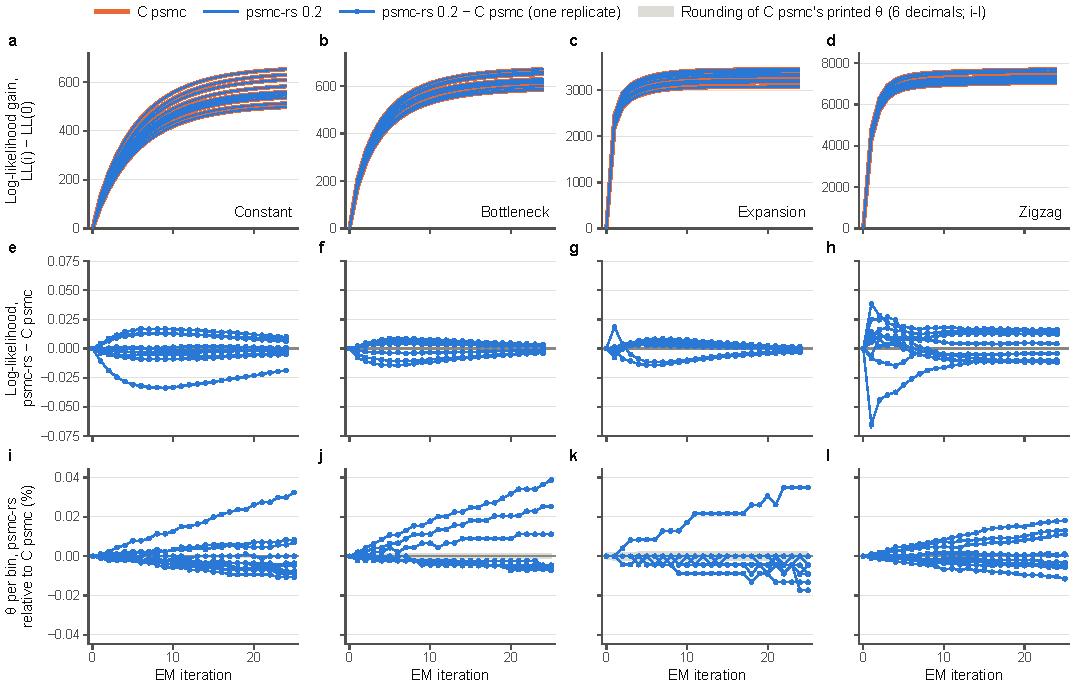
\includegraphics[width=\linewidth]{E1/figures/figS1_em_convergence.pdf}
\caption{EM convergence of C psmc and \psmcrs{} 0.2 on the same genomes (E1). One column per model; every replicate is a line. Iteration $i$ counts completed EM iterations: C psmc's log-likelihood of round $i+1$ and \psmcrs{}'s after $i$ iterations are both the log-likelihood after $i$ iterations. C psmc prints none after its last iteration, so both programs' log-likelihoods are drawn up to the last iteration both give. (a--d) Log-likelihood gained since the start, $\mathrm{LL}(i)-\mathrm{LL}(0)$, for both programs (C psmc wider, underneath). (e--h) \psmcrs{}'s log-likelihood minus C psmc's after the same iteration (log-likelihood units; iteration 0 evaluates the same starting model). (i--l) $\theta$ per bin of \psmcrs{} relative to C psmc's after each iteration, in percent. C psmc prints $\theta$ to six decimals, so its $\theta$ is known only to $\pm0.5\times10^{-6}$: the grey band is that rounding, relative to C psmc's smallest $\theta$ of the model at each iteration, and the steps of the lines are its quanta. The log-likelihood did not decrease between iterations in any of the \EoneRuns{} fits.}
\label{fig:s1}
\end{figure}

\begin{figure}[p]
\centering
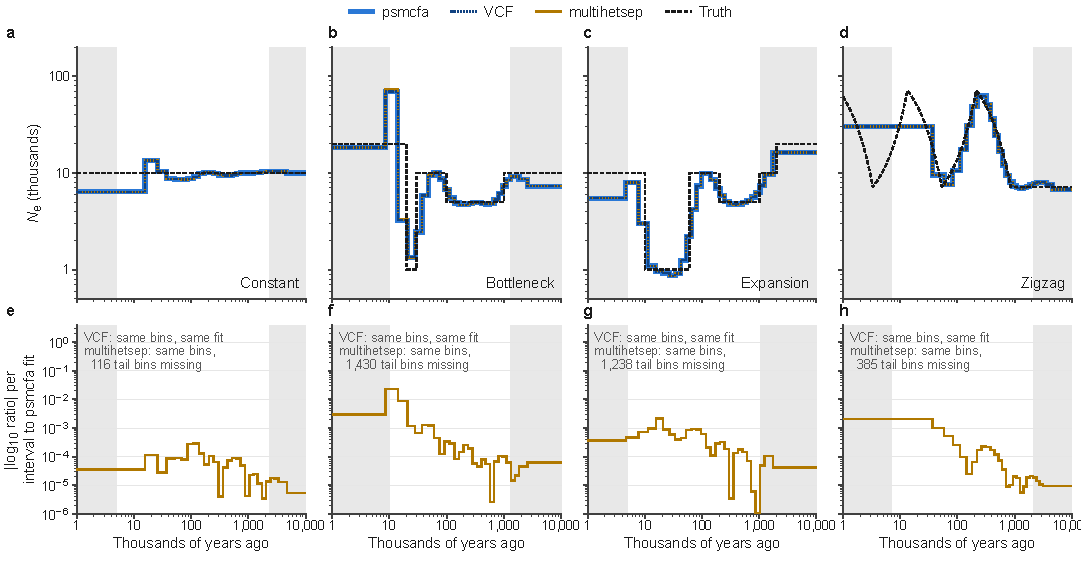
\includegraphics[width=\linewidth]{E6/figures/figS2_format_consistency.pdf}
\caption{One simulated genome per model read as \texttt{psmcfa}, VCF and multihetsep (E6). E1's first replicate of each model, without missing data, in the three formats, fitted by \psmcrs{} 0.2 with E1's settings. (a--d) The three fits and the truth: the \texttt{psmcfa} fit wide, underneath; the multihetsep fit thin and solid over it; the VCF fit dotted on top (it equals the \texttt{psmcfa} fit, so its dots run along the wide line). (e--h) $|\log_{10}(\Ne/\Ne^{\texttt{psmcfa}})|$ interval by interval for the VCF and multihetsep inputs, drawn as a step curve on the \texttt{psmcfa} fit's intervals (log scale); an input whose fit equals the \texttt{psmcfa} fit exactly is named instead of drawn. Each panel gives the bins that differ from the \texttt{psmcfa} file's (none) and the bins after the last heterozygous site, which a multihetsep file, ending at its last row, lacks (\EsixMhsTailMin{} to \EsixMhsTailMax{} per genome); the multihetsep fits differed by at most \EsixMhsMaxAbs{} in $\log_{10}\Ne$.}
\label{fig:s2}
\end{figure}

\begin{figure}[p]
\centering
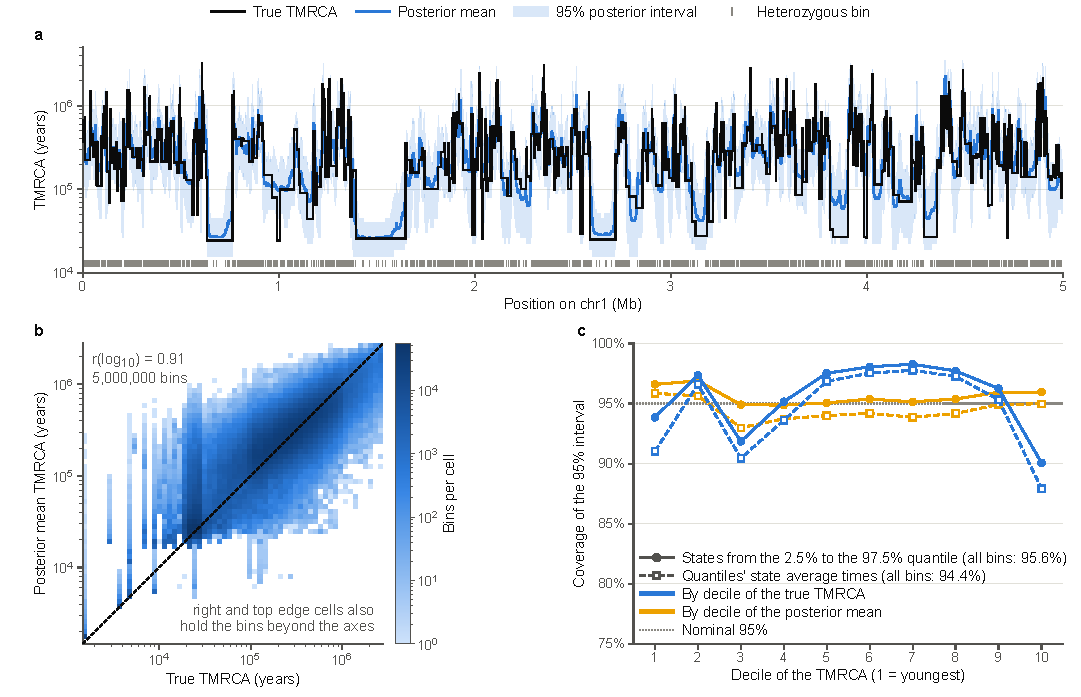
\includegraphics[width=\linewidth]{E6/figures/figS3_tmrca_decoding.pdf}
\caption{Posterior TMRCA decoding against the true pairwise TMRCA (E6). E1's first bottleneck replicate (\EsixDecodeBins{} bins) decoded by \psmcrs{} 0.2 with its fitted model (\opt{--tmrca-out}); the true TMRCA of every 100~bp bin comes from the tree sequence, re-simulated from the replicate's seeds. (a) An example window, the first 5~Mb of chromosome~1: the true TMRCA (black), the posterior mean (blue) and its 95\% interval (band); ticks mark the heterozygous bins. (b) The posterior mean against the true TMRCA over every bin, as a two-dimensional histogram (log counts), with the identity line and the correlation of the logarithms ($r=$~\EsixDecodeR{}). The grid runs from the youngest true TMRCA to the 99.95\% quantile of both variables, and bins beyond it are counted in the edge cells. Each vertical streak is a stretch of many bins that share one true TMRCA (one long genealogical segment, or a few); along a streak the posterior moves across the segment's ends. (c) Share of bins whose 95\% interval holds the true TMRCA, by decile of the true TMRCA (blue) and by decile of the posterior mean (yellow): the interval of PSMC states from the 2.5\% to the 97.5\% posterior quantile (solid, filled circles) and the quantiles' state average times (dashed, open squares), against the nominal 95\%. By decile of the true TMRCA the coverage of the states' interval ranged from \EsixTrueDecileMin{}, in the oldest decile, where the posterior mean was too young by \EsixOldBias{} in $\log_{10}$ on average, to \EsixTrueDecileMax{} (in the youngest decile the posterior mean was too old by \EsixYoungBias{}); by decile of the posterior mean, what an analysis sees, it ranged from \EsixPostDecileMin{} to \EsixPostDecileMax{}.}
\label{fig:s3}
\end{figure}

\begin{figure}[p]
\centering
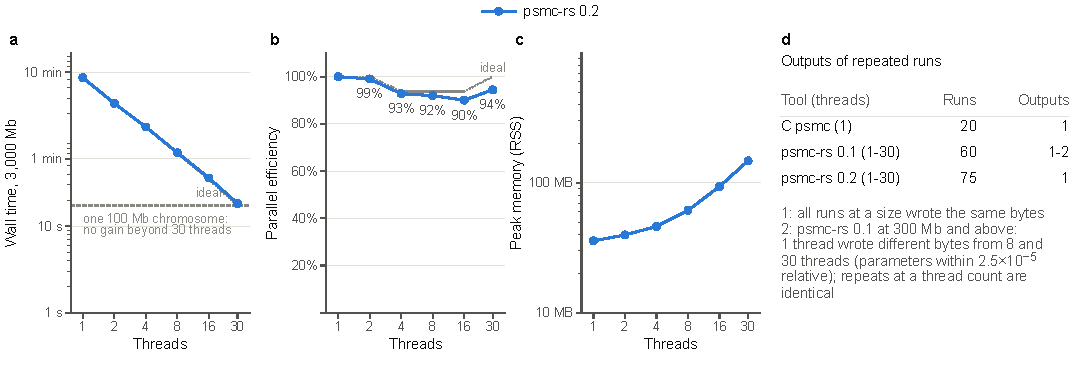
\includegraphics[width=\linewidth]{E3/figures/figS4_thread_scaling.pdf}
\caption{Thread scaling and determinism of \psmcrs{} 0.2 (E3). On the \EthreeBigMb{}~Mb genome (\EthreeBigChroms{} chromosomes of 100~Mb, 25 EM iterations), on 1 to 30 threads. (a) Wall time against threads: every repeat (dots) and the median (line), with ideal scaling from the fewest threads (dotted). The M-step runs on one thread but converges in a few milliseconds per EM iteration, so the E-step's sequences set the speed-up. \psmcrs{} works on one sequence per thread, so the ideal is that of whole sequences per thread (30 sequences on 8 threads take 4 rounds, a speed-up of 7.5), and its floor, marked, is the time of one chromosome. (b) Parallel efficiency, speed-up over threads, of the medians (\EthreeEffMin{} to \EthreeEffMax{}), and the ideal's (dotted): 1 where the threads divide the sequences, \EthreeEffCap{} on 4, 8 and 16 threads. (c) Peak memory of the process tree against threads. (d) Determinism, per program, with its thread counts in brackets: Runs, the runs summed over E3's four genome sizes; Outputs, how many distinct output files the runs at one genome size wrote. \psmcrs{} 0.1 on one thread wrote different bytes than on 8 and 30 threads at 300~Mb and above (parameters within a relative \EthreeRsZeroDiffMax{}), while its repeats at one thread count were identical.}
\label{fig:s4}
\end{figure}

\begin{figure}[p]
\centering
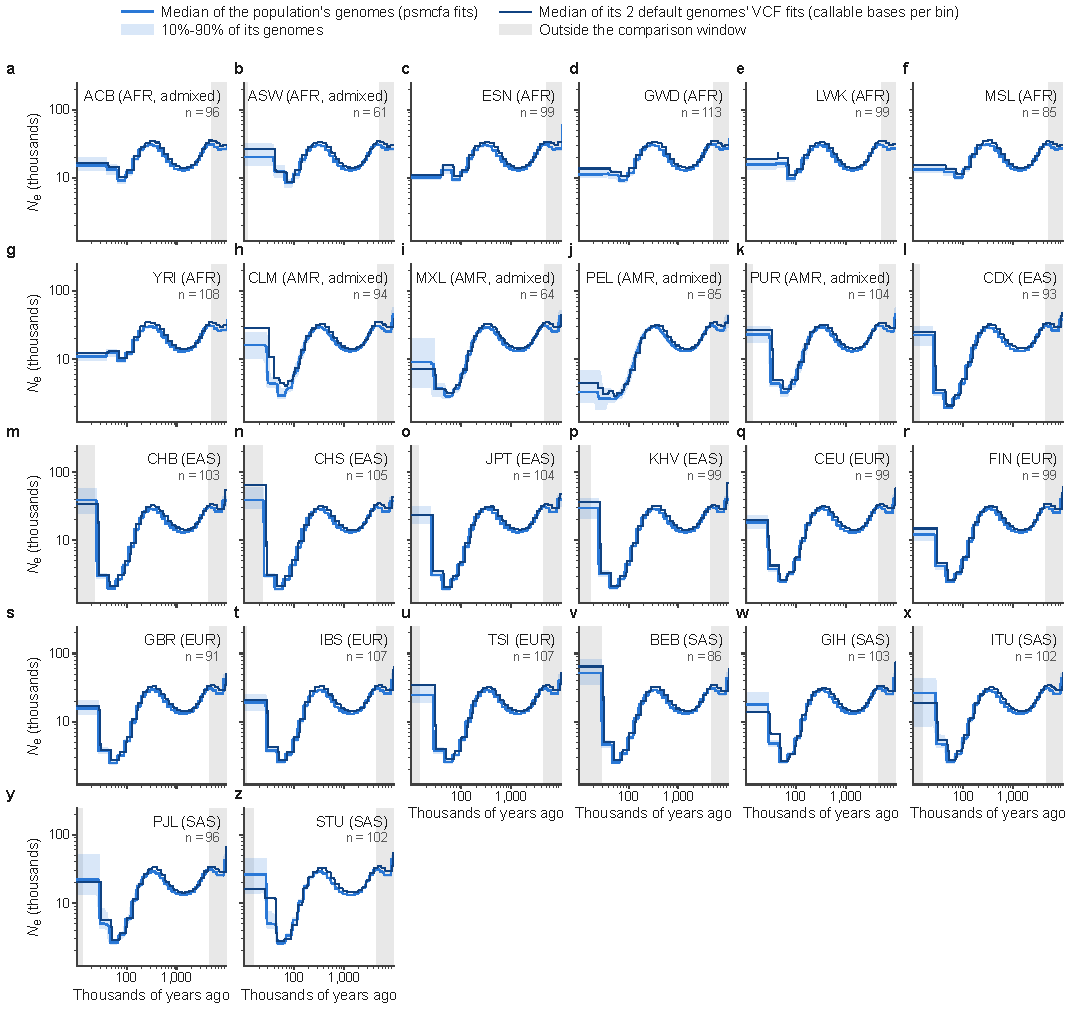
\includegraphics[width=\linewidth]{E7/figures/figS5_1000g_populations.pdf}
\caption{Every population of the 1000 Genomes data and the spread between its genomes (E7). One panel per population, ordered by superpopulation: the median of the population's genomes (fits of their \texttt{psmcfa} files; blue; the population's curve in Fig.~7a--e) with the spread between them (10\% to 90\%, a band of individuals, not a confidence interval; $n$, the genomes, in the panel), and the median of the VCF fits (the strict mask, callable bases per bin) of its two default genomes (dark blue, thin). A \texttt{psmcfa} file records no callable bases per bin, so its fit takes every called bin as full (\EsevenMissingShare{} of the called bins' bases are missing here), which makes $\theta$, and every size and time, low (Fig.~5). On the same genome the VCF fit's $\theta$ is \EsevenThetaShift{} higher (\EsevenThetaShiftLo{} to \EsevenThetaShiftHi{} over the \EsevenDefault{} default genomes) and its \Ne{} \EsevenNeShift{} higher in $\log_{10}$ on average over the window at the same times (Fig.~S6b): the dark line runs above, and slightly later than, the blue one. In the first time window two genomes are a small sample of a wide spread, and the dark line strays to either side of the blue one. All panels share their axes. Times outside the population's median comparison window are shaded. Admixed populations are marked. $\mu=\EsevenMu$ per bp per generation, $g=\EsevenG$ years.}
\label{fig:s5}
\end{figure}

\begin{figure}[p]
\centering
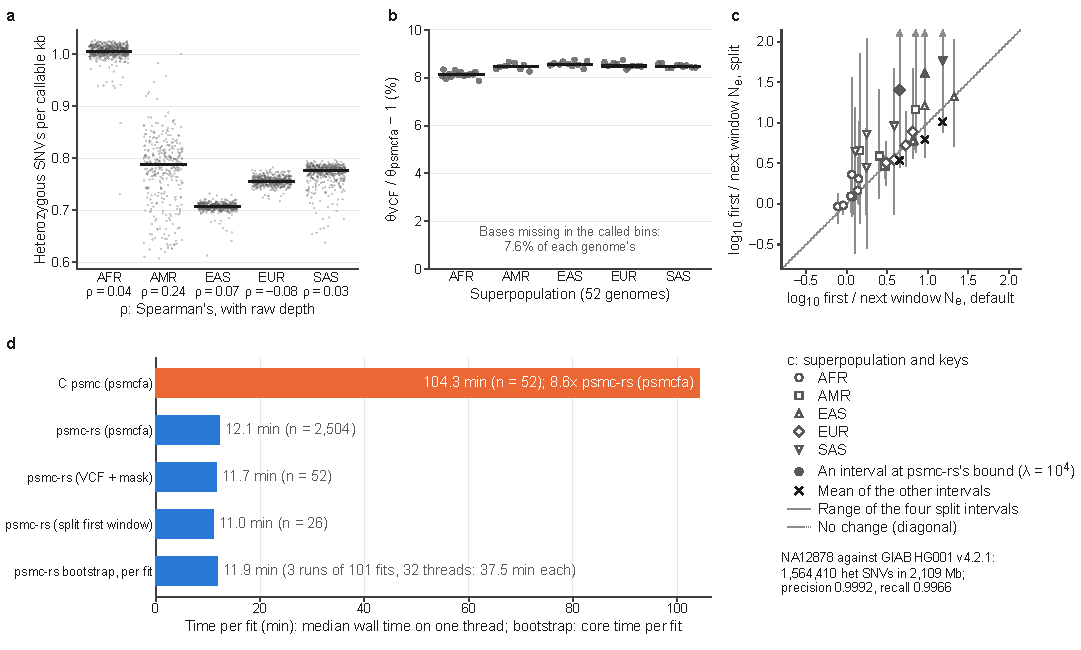
\includegraphics[width=\linewidth]{E7/figures/figS6_1000g_checks.pdf}
\caption{The 1000 Genomes inputs and checks (E7). (a) Heterozygous single-nucleotide sites per callable kb of every genome of the cohort, by superpopulation (points jittered sideways; the line is the median); under each superpopulation, Spearman's $\rho$ between heterozygosity and raw sequencing depth among its genomes. (b) The two routes on the default set (\EsevenDefault{} genomes): $\theta$ of the VCF fit (the strict mask, callable bases per bin) over $\theta$ of the \texttt{psmcfa} fit of the same genome, minus one, by superpopulation. The VCF fit's $\theta$ is \EsevenThetaShift{} higher on average (\EsevenThetaShiftLo{} to \EsevenThetaShiftHi{}), because the \texttt{psmcfa} fit takes every called bin as full and the bases missing from the called bins (\EsevenMissingShare{}) make $\theta$ low (Fig.~5). (c) The split-first-window check \citep{hilgers2025}: the first window's \Ne{} over the next window's, under the default pattern ($x$) and with the first window split into its four intervals ($y$; their $\log_{10}\Ne$ averaged by duration, the vertical line their range); a point on the diagonal did not move, and a range that runs past the top ends in an arrow. Filled markers: genomes whose split fit put one first-window interval at \psmcrs{}'s upper bound on a free $\lambda$ (\EsevenSplitBound{} of \EsevenSplitN{}), where one genome barely constrains such a short interval; the cross is the duration-weighted mean of their other intervals. (d) Time per fit of every route: single-thread fits by their median wall time; \psmcrs{}'s bootstrap (a main fit and \EsevenBootReps{} replicates per run on \EsevenBootThreads{} threads; \EsevenBootSamplesW{} runs) by its median wall time times its threads over its fits, the core time of one of its fits. On one thread of the same shared node, \psmcrs{} fitted the same \texttt{psmcfa} \EsevenSpeed{} times as fast as C psmc. The note under the legend gives NA12878's heterozygous single-nucleotide sites against Genome in a Bottle's HG001 v4.2.1 benchmark inside the strict mask and the benchmark's regions (precision \EsevenGiabPrecision{}, recall \EsevenGiabRecall{}).}
\label{fig:s6}
\end{figure}

\begin{figure}[p]
\centering
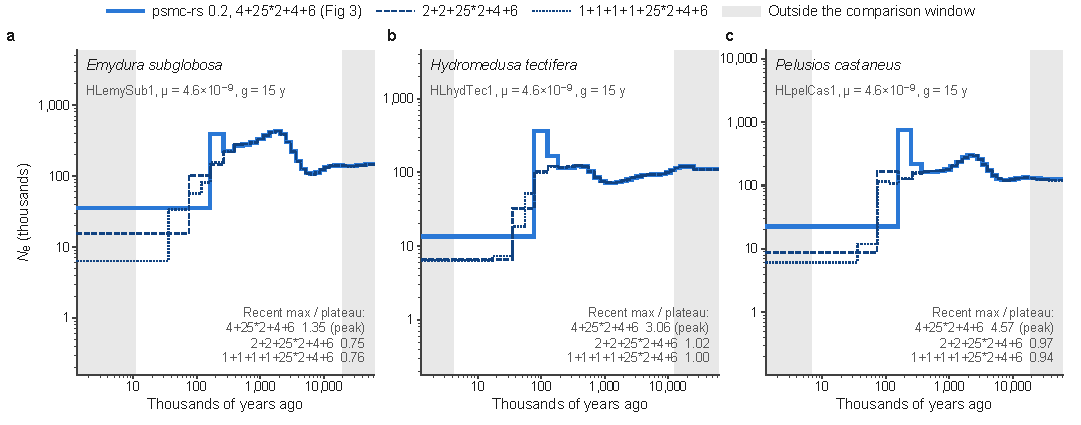
\includegraphics[width=\linewidth]{E2/figures/figS_turtle_patterns.pdf}
\caption{The split-first-window check of the three turtles (E2). \citet{hilgers2025} found false recent peaks of \Ne{} in PSMC curves across many studies under the pattern \opt{4+25*2+4+6} that Fig.~3 uses, whose first free $\lambda$ spans the first four of the 64 intervals; splitting that window removed the peaks. One panel per turtle: \psmcrs{}'s fit of Fig.~3 (\opt{4+25*2+4+6}; blue, wider, underneath) and its fits of the same input with the first window split in two (\opt{2+2+25*2+4+6}; dark blue, dashed) and in four (\opt{1+1+1+1+25*2+4+6}; dark blue, dotted), every other setting the same. Curves are scaled as in Fig.~3. Times outside the comparison window of Fig.~3 are shaded. The note gives, for each pattern, the largest \Ne{} of the recent intervals (the first eight) relative to the plateau (the median \Ne{} of the next eight), and ``peak'' where the largest lies after the first interval and is at least 1.25 times both the first interval's \Ne{} and the plateau: \EtwoPeaksDefaultW{} of the \EtwoTurtlesW{} fits under the default pattern (\EtwoPeakMin{} to \EtwoPeakMax{} times the plateau) and \EtwoPeaksSplitW{} of the \EtwoSplitFitsW{} split fits.}
\label{fig:s7}
\end{figure}

\clearpage
\section{Supplementary Table}

\begin{table}[h]
\centering\scriptsize
\caption{Checks of E2's four genomes by \opt{psmc-rs qc} (E6), with 100~bp bins and bootstrap blocks of 500,000 bins: sequences; called bases; share of bins missing; heterozygosity per kb estimated from the share of heterozygous bins; N50 of the sequences; share of heterozygous bins expected to hold two or more heterozygous sites (\texttt{BIN\_SATURATION} above 10\%); share of bins in sequences shorter than a bootstrap block (\texttt{SHORT\_SEQUENCES} above 20\%); and the warnings raised.}
\label{tab:s1}
\setlength{\tabcolsep}{3pt}
\begin{tabular}{@{}lrrrrrrrr>{\raggedright\arraybackslash}p{2.9cm}@{}}
\toprule
Genome & Sequences & \begin{tabular}[b]{@{}c@{}}Called \\ (Gb)\end{tabular} & Missing & \begin{tabular}[b]{@{}c@{}}Het \\ per kb\end{tabular} & \begin{tabular}[b]{@{}c@{}}N50 \\ (Mb)\end{tabular} & \begin{tabular}[b]{@{}c@{}}K bins with \\ $\geq$2 het\end{tabular} & \begin{tabular}[b]{@{}c@{}}Bin size for \\ $<$5\% (bp)\end{tabular} & \begin{tabular}[b]{@{}c@{}}Bins in \\ short seq.\end{tabular} & Warnings \\
\midrule
\textit{H. sapiens} (NA12878) & 22 & 2.34 & 18.6\% & 0.65 & 145.1 & 3.2\% & 157 & 2\% & -- \\
\textit{E. subglobosa} & 889 & 1.88 & 2.3\% & 2.55 & 44.8 & 12.1\% & 40 & 50\% & BIN\_SATURATION, SHORT\_SEQUENCES \\
\textit{H. tectifera} & 34 & 1.84 & 0.5\% & 1.41 & 118.6 & 6.8\% & 73 & 23\% & SHORT\_SEQUENCES \\
\textit{P. castaneus} & 1,220 & 1.87 & 3.8\% & 2.39 & 14.9 & 11.4\% & 43 & 97\% & BIN\_SATURATION, SHORT\_SEQUENCES \\
\bottomrule
\end{tabular}

\end{table}

\clearpage
{\sloppy% Generated by manuscript/make_sn1.py from experiment/Supplementary_Note_1_Reproducibility.md; do not edit.
\section{Supplementary Note 1 --- Reproducibility}\label{supplementary-note-1-reproducibility}

This note describes how to reproduce the manuscript's experiments, tables
and figures from the \texttt{psmc-rs} repository: from the committed results
without running any tool, from scratch on one machine, or on a SLURM
cluster, as the production runs were made. It also says how every output
records the way it was made, how C psmc was built, and which results do
not depend on the thread count or the CPU. Paths are relative to the
repository root. The pipeline itself is described in
\texttt{experiment/\allowbreak{}pipeline/\allowbreak{}README.md}, the figures in
\texttt{experiment/\allowbreak{}pipeline/\allowbreak{}figures/\allowbreak{}README.md} and the cluster scripts in
\texttt{experiment/\allowbreak{}slurm/\allowbreak{}README.md}.

The experiments are E1 (simulated accuracy and agreement with C psmc:
Fig 1, Table 1, Table S1, Fig S1), E2 (four real genomes: Fig 1, Table 1),
E3 (performance: Fig 2, Table 2), E4 (partly callable bins: Fig S2), E5
(bootstrap calibration: Fig S3), E6 (supplementary analyses, quoted in the
text) and E7 (the 1000 Genomes 30x genomes: Fig 3, Fig 1, Fig 2c, Table 1); FIG
draws every figure. The pipeline names most figure files after an earlier
plan of the article, and draws some that the article leaves out; section
3 maps them.

\subsection{1) What the repository holds}\label{what-the-repository-holds}

Each experiment writes \texttt{experiment/\allowbreak{}runs/\allowbreak{}\textless{}EXP\textgreater{}/\allowbreak{}}. The repository holds the
production runs of E1 to E7 and FIG:

{\def\LTcaptype{none} % do not increment counter
\begin{longtable}[]{@{}
  >{\raggedright\arraybackslash}p{(\linewidth - 2\tabcolsep) * \real{0.5000}}
  >{\raggedright\arraybackslash}p{(\linewidth - 2\tabcolsep) * \real{0.5000}}@{}}
\toprule\noalign{}
\begin{minipage}[b]{\linewidth}\raggedright
item
\end{minipage} & \begin{minipage}[b]{\linewidth}\raggedright
where
\end{minipage} \\
\midrule\noalign{}
\endhead
\bottomrule\noalign{}
\endlastfoot
real genomes (inputs of E2 and E6's S5): the three turtles, and NA12878's chr1-22, E7's psmcfa of that sample byte for byte (its SHA-256 is in E7's \texttt{MANIFEST.json} and \texttt{config.RealGenome.sha256}) & \texttt{experiment/\allowbreak{}real\_\allowbreak{}data/\allowbreak{}\{HLemySub1,\allowbreak{}HLhydTec1,\allowbreak{}HLpelCas1\}\_\allowbreak{}diploid.psmcfa}, \texttt{experiment/\allowbreak{}real\_\allowbreak{}data/\allowbreak{}NA12878\_\allowbreak{}1kGP30x\_\allowbreak{}diploid.psmcfa.gz} (\texttt{Papuan\_\allowbreak{}highlands\_\allowbreak{}diploid.psmcfa}, a chromosome 1, serves the README's benchmarks and the Rust tests; E2 does not read it) \\
truth records of the simulated genomes (settings, seeds, software versions, per-chromosome counts and checksums, the true Ne(t)) & \texttt{runs/\allowbreak{}\textless{}EXP\textgreater{}/\allowbreak{}truth/\allowbreak{}} \\
every fit: psmc-rs JSON and \texttt{.psmc}, C psmc \texttt{.psmc} & \texttt{runs/\allowbreak{}\textless{}EXP\textgreater{}/\allowbreak{}fits/\allowbreak{}} \\
bootstrap runs: main fit, every replicate's JSON, \texttt{summary.json} and \texttt{summary.tsv} & \texttt{runs/\allowbreak{}E2/\allowbreak{}bootstrap/\allowbreak{}}, \texttt{runs/\allowbreak{}E5/\allowbreak{}boot/\allowbreak{}}, \texttt{runs/\allowbreak{}E7/\allowbreak{}boot/\allowbreak{}} \\
E4's masks, bins and cross-checks; QC reports & \texttt{runs/\allowbreak{}E4/\allowbreak{}\{masks,\allowbreak{}bins,\allowbreak{}consensus,\allowbreak{}crosscheck\}/\allowbreak{}}, \texttt{runs/\allowbreak{}\{E2,\allowbreak{}E6\}/\allowbreak{}qc/\allowbreak{}} \\
one provenance record per job & \texttt{runs/\allowbreak{}\textless{}EXP\textgreater{}/\allowbreak{}provenance/\allowbreak{}} \\
tables and figures & \texttt{runs/\allowbreak{}\textless{}EXP\textgreater{}/\allowbreak{}tables/\allowbreak{}}, \texttt{runs/\allowbreak{}\textless{}EXP\textgreater{}/\allowbreak{}figures/\allowbreak{}} (the software's schematic, not in the article: \texttt{runs/\allowbreak{}FIG/\allowbreak{}}) \\
E7's inputs: one psmcfa per 1000 Genomes sample (the strict mask applied, non-PASS positions missing), the default set's het-or-missing VCFs and the masks & Zenodo, not the repository (\texttt{runs/\allowbreak{}E7/\allowbreak{}inputs/\allowbreak{}}; remade by \texttt{python\ -m\ experiment.pipeline.kg1000}) \\
E7's data stage: \texttt{MANIFEST.json} (sources, tool versions, commands, checks, SHA-256 of every file it wrote) and its records (how each chromosome was read, its chunks, the chr21 pilot as the stage ran it); the chr21 pilot and the default genomes' conversions redone with the production's psmc-rs & \texttt{runs/\allowbreak{}E7/\allowbreak{}inputs/\allowbreak{}MANIFEST.json}, \texttt{runs/\allowbreak{}E7/\allowbreak{}inputs/\allowbreak{}records/\allowbreak{}}, \texttt{experiment/\allowbreak{}e7\_\allowbreak{}pilot/\allowbreak{}} \\
the analyses outside the pipeline, each with its scripts, results and README: the cross-platform comparison (section 9) and the diagnostic of the residual difference from C psmc (variants of psmc-rs, as a patch, and their fits of E1's genomes) & \texttt{experiment/\allowbreak{}crossplatform/\allowbreak{}}, \texttt{experiment/\allowbreak{}c\_\allowbreak{}equivalence/\allowbreak{}} \\
\end{longtable}
}

Not committed, and remade on demand from the seeds: the simulated genomes
(psmcfa, VCF, true TMRCA tracks; \texttt{runs/\allowbreak{}*/\allowbreak{}sims/\allowbreak{}}), the bootstrap
replicates' \texttt{.psmc} files, HTML reports, logs and the runner's state
(\texttt{runs/\allowbreak{}\_\allowbreak{}runner/\allowbreak{}}).

\subsection{2) Software}\label{software}

\begin{itemize}
\tightlist
\item
  \textbf{Python} 3.13.13 with the exact packages of
  \texttt{experiment/\allowbreak{}pipeline/\allowbreak{}requirements.lock} (msprime 1.4.4, tskit 1.0.3,
  numpy 2.5.3, stdpopsim 0.3.0, scipy 1.18.1, pandas 3.0.6, matplotlib
  3.11.2, \ldots), and htslib 1.24 (\texttt{bgzip}, \texttt{tabix}, \texttt{bcftools}). The
  simulations are byte-identical only with these versions, which every
  truth record lists; \texttt{python\ -m\ experiment.pipeline\ tools} and \texttt{start}
  warn when the running interpreter differs.
\item
  \textbf{psmc-rs 0.2.0}, built from the repository with \texttt{cargo\ build\ -\/\allowbreak{}-release\ -\/\allowbreak{}-locked} (Rust 1.88 or later; the production build used rustc 1.99.0,
  the release profile and no \texttt{RUSTFLAGS}).
\item
  \textbf{C psmc} (lh3/psmc 0.6.5-r74) with its \texttt{fq2psmcfa} and \texttt{splitfa},
  and \texttt{generate\_\allowbreak{}multihetsep.py} of msmc-tools, in \texttt{experiment/\allowbreak{}.tools} (or
  \texttt{\$PSMC\_\allowbreak{}EXP\_\allowbreak{}TOOLS}); section 7 describes the builds.
\item
  \textbf{Figures:} Arial (else Helvetica, else DejaVu Sans).
\end{itemize}

\begin{verbatim}
git clone https://github.com/larryivan/psmc-rs.git && cd psmc-rs
git checkout <MANUSCRIPT_TAG>
python3.13 -m venv experiment/.venv
experiment/.venv/bin/python -m pip install -r experiment/pipeline/requirements.lock
cargo build --release --locked
T=experiment/.tools
git clone https://github.com/lh3/psmc $T/psmc_c && git -C $T/psmc_c checkout 82fa2ad
git clone https://github.com/stschiff/msmc-tools $T/msmc-tools
PY=experiment/.venv/bin/python
$PY -m experiment.pipeline tools --build-c   # builds C psmc; exits 1 if a tool is missing
\end{verbatim}

\subsection{3) Tables and figures from the committed results}\label{tables-and-figures-from-the-committed-results}

No tool runs for these. Each experiment's report reads the committed
fits, bootstrap files, truth and QC records and writes its tables; the
figures are drawn from the tables:

\begin{verbatim}
$PY -m experiment.pipeline report E1     # likewise E2, E4, E5
$PY -m experiment.pipeline report E6     # S1 and S5; S2 and S3 need the simulated genomes (section 4)
$PY -m experiment.pipeline.figures       # every figure whose tables exist, into runs/<EXP>/figures/
\end{verbatim}

\texttt{python\ -m\ experiment.pipeline.figures\ -\/\allowbreak{}-list} names the tables each
figure reads. The article's figures and tables are these files of the
runs (\texttt{manuscript/\allowbreak{}make\_\allowbreak{}numbers.py} writes the tables' LaTeX):

{\def\LTcaptype{none} % do not increment counter
\begin{longtable}[]{@{}
  >{\raggedright\arraybackslash}p{(\linewidth - 2\tabcolsep) * \real{0.5000}}
  >{\raggedright\arraybackslash}p{(\linewidth - 2\tabcolsep) * \real{0.5000}}@{}}
\toprule\noalign{}
\begin{minipage}[b]{\linewidth}\raggedright
article
\end{minipage} & \begin{minipage}[b]{\linewidth}\raggedright
file
\end{minipage} \\
\midrule\noalign{}
\endhead
\bottomrule\noalign{}
\endlastfoot
Fig 1 & \texttt{runs/\allowbreak{}FIG/\allowbreak{}figures/\allowbreak{}art1\_\allowbreak{}agreement} (from E1, E2 and E7's tables) \\
Fig 2 & \texttt{runs/\allowbreak{}E3/\allowbreak{}figures/\allowbreak{}art2\_\allowbreak{}performance} (from E3 and E7's tables) \\
Fig 3 & \texttt{runs/\allowbreak{}E7/\allowbreak{}figures/\allowbreak{}fig7\_\allowbreak{}1000\_\allowbreak{}genomes} \\
Table 1 & from \texttt{E1\_\allowbreak{}rs\_\allowbreak{}vs\_\allowbreak{}c}, \texttt{E1\_\allowbreak{}replicates}, \texttt{E2\_\allowbreak{}rs\_\allowbreak{}vs\_\allowbreak{}c}, \texttt{E2\_\allowbreak{}fit\_\allowbreak{}summary}, \texttt{E7\_\allowbreak{}rs\_\allowbreak{}vs\_\allowbreak{}c} and \texttt{E7\_\allowbreak{}fits} \\
Table 2 & \texttt{runs/\allowbreak{}E3/\allowbreak{}tables/\allowbreak{}E3\_\allowbreak{}table2.csv} \\
Fig S1 & \texttt{runs/\allowbreak{}E1/\allowbreak{}figures/\allowbreak{}figS1\_\allowbreak{}em\_\allowbreak{}convergence} \\
Fig S2 & \texttt{runs/\allowbreak{}E4/\allowbreak{}figures/\allowbreak{}fig5\_\allowbreak{}input\_\allowbreak{}preparation} \\
Fig S3 & \texttt{runs/\allowbreak{}E5/\allowbreak{}figures/\allowbreak{}fig6\_\allowbreak{}bootstrap\_\allowbreak{}calibration} \\
Table S1 & \texttt{runs/\allowbreak{}E1/\allowbreak{}tables/\allowbreak{}E1\_\allowbreak{}table1.csv} \\
\end{longtable}
}

The pipeline also draws figures that the article leaves out, for the
analyses it quotes in its text: the software's schematic
(\texttt{runs/\allowbreak{}FIG/\allowbreak{}figures/\allowbreak{}fig1\_\allowbreak{}workflow}), E1's and E2's fits in more detail
(\texttt{runs/\allowbreak{}E1/\allowbreak{}figures/\allowbreak{}fig2\_\allowbreak{}simulated\_\allowbreak{}accuracy},
\texttt{runs/\allowbreak{}E2/\allowbreak{}figures/\allowbreak{}fig3\_\allowbreak{}real\_\allowbreak{}genomes}), E3's timings at every size and
thread count of section 10 and its thread scaling
(\texttt{runs/\allowbreak{}E3/\allowbreak{}figures/\allowbreak{}fig4\_\allowbreak{}performance}, \texttt{figS4\_\allowbreak{}thread\_\allowbreak{}scaling}), E6's format consistency and TMRCA decoding
(\texttt{runs/\allowbreak{}E6/\allowbreak{}figures/\allowbreak{}figS2\_\allowbreak{}format\_\allowbreak{}consistency}, \texttt{figS3\_\allowbreak{}tmrca\_\allowbreak{}decoding}),
E2's split-first-window check (\texttt{runs/\allowbreak{}E2/\allowbreak{}figures/\allowbreak{}figS\_\allowbreak{}turtle\_\allowbreak{}patterns})
and E7's populations and checks
(\texttt{runs/\allowbreak{}E7/\allowbreak{}figures/\allowbreak{}figS5\_\allowbreak{}1000g\_\allowbreak{}populations}, \texttt{figS6\_\allowbreak{}1000g\_\allowbreak{}checks}). The
numbers in the article's text and tables, and the counts in Fig 1, come
from the same tables through \texttt{manuscript/\allowbreak{}make\_\allowbreak{}numbers.py}.

E6's S2 compares the fits of E1's first replicates read as psmcfa, VCF and
multihetsep, and reads the simulated psmcfa to count the bins; S3 compares
the decoded TMRCA with the true one re-simulated from the replicate's
seeds. Both need the simulated genomes, which section 4 regenerates.

The analysis does not depend on the platform beyond its last digits.
The reports of E1, E2, E4 and E5, run on an Apple M1 Pro laptop (macOS,
arm64) on the committed fits, with the code that wrote the committed
tables on the Ibex cluster (Linux, x86-64) in the production of section 5
(the same code digests and package versions), wrote 16 of the 38 tables
byte for byte; the others agreed with those written on Ibex to a relative
2.5e-13 in every value of magnitude 1e-3 or more, and to a relative
1.9e-11 in the differences between psmc-rs and C psmc, of order 1e-5 (at
most 8.9e-16 absolute); the differences come from the two platforms' math
libraries (\texttt{experiment/\allowbreak{}crossplatform/\allowbreak{}summary.md}, section 4.6).

\subsection{4) The runs, on one machine}\label{the-runs-on-one-machine}

The pipeline is a job graph run by a detached, resumable runner (the
Runner section of \texttt{experiment/\allowbreak{}pipeline/\allowbreak{}README.md}). Into a fresh runs
directory, to reproduce E1, E4, E5 and E6 from scratch (E2 and E3 below;
E7 needs its inputs, section 1):

\begin{verbatim}
RUNS=/path/to/new/runs
$PY -m experiment.pipeline plan                       # estimated CPU hours and wall time
$PY -m experiment.pipeline start --runs-dir $RUNS E1 E4 E5 E6 FIG
$PY -m experiment.pipeline status --runs-dir $RUNS    # done/running/failed/pending, ETA
$PY -m experiment.pipeline stop --runs-dir $RUNS      # any time; `start` again resumes
\end{verbatim}

FIG draws the figures into \texttt{\$RUNS} once their tables exist, and comparing
the tables of \texttt{\$RUNS} with the committed ones shows what was reproduced.

\texttt{-\/\allowbreak{}-cores} and \texttt{-\/\allowbreak{}-mem-gb} set the runner's budget (default 7 cores and
12 GB). E2's bootstraps run on 50 threads each, so E2 needs \texttt{-\/\allowbreak{}-cores\ 50}
and a machine with at least 50 cores; E3 needs the machine to itself
(\texttt{start\ E3} on a quiet machine on AC power; see the pipeline README's E3
section). On the development laptop (Apple M1 Pro, 8 cores,
16 GB), \texttt{plan} estimates E1 at 1.4 hours, E4 at 0.6, E5 at 2.3 and E6 at
0.1 (wall time alone on 7 cores). Section 5 gives the costs measured in
the production run.

In the repository's own \texttt{experiment/\allowbreak{}runs}, where the results are
committed, a job counts as done when its outputs exist and its provenance
record matches: the same command, settings, seeds, input checksums and tool
identities (section 6). Inputs count by content, so a simulation that
reproduces its recorded checksums leaves the jobs that read it done. With
the production's tools, \texttt{start\ E1\ E6} would therefore remake only what is
not committed: the simulated genomes, S2's conversions and S3's true and
decoded TMRCA tracks. \texttt{report\ E6} then writes their tables. With other builds of the tools (for
example psmc-rs built by another rustc, or another C psmc binary) their
fits count as not done and run again; \texttt{status\ -\/\allowbreak{}-jobs} lists what \texttt{start}
would run, and \texttt{start\ -\/\allowbreak{}-only\ REGEX} restricts it to the matching jobs.

\subsection{5) The runs, on a SLURM cluster}\label{the-runs-on-a-slurm-cluster}

The production runs of E1 to E7 were made with the scripts of
\texttt{experiment/\allowbreak{}slurm/\allowbreak{}} on KAUST's Ibex cluster (E3's repeats as \texttt{e3} jobs,
section 10; E7's data stage as \texttt{e7-prep}), and the figures drawn on the
laptop from the runs directory copied back. The scripts run the same pipeline in SLURM allocations;
site settings (account, partition, node constraints, paths, C psmc's
flags) go in \texttt{experiment/\allowbreak{}slurm/\allowbreak{}site.env}, copied from
\texttt{site.env.example}. Every job sources \texttt{env.sh}, which gives it
one environment whatever shell submitted it: the pinned Rust toolchain
without build flags, the Python environment with its htslib first on
\texttt{PATH}, the tools directory, and a machine lock in the job's own \texttt{/\allowbreak{}tmp}.

\begin{verbatim}
cd $PROD/experiment/slurm          # $PROD: a dedicated worktree of the production commit
./submit.sh build                  # build psmc-rs 0.2 and C psmc, run every Rust and Python test
./submit.sh prod                   # E1 E2 E4 E5 E6 in one allocation; submit again if the time ran out
./submit.sh e3 1 2 3 4 5           # E3: one exclusive node of one CPU model per repeat
./merge_e3.sh                      # once every e3 job has ended
./submit.sh e3-report              # E3's tables
./submit.sh e7-prep                # E7's inputs from the 1000 Genomes VCFs; then prod again for E7's fits
\end{verbatim}

The production ran in two \texttt{prod} jobs of commit 4b2c636. The first
(SLURM job 54256959, on node cn513-11-l on 22 and 23 October 2026; 5 hours
53 minutes) ran every job whose key the code had changed: the psmc-rs
fits, bootstraps, conversions, decoding and QC of E1, E2 and E4 to E6,
E4's cross-checks, and the reports of E1, E2, E4 and E5. The second
(54555780, on node cn514-10-l on 25 and 26 October) ran every fit and
bootstrap of E7, C psmc's and psmc-rs's together, so that their times
compare like for like, and E7's report. The jobs whose keys had not
changed were kept from earlier jobs: the C psmc fits of E1 and the
turtles (53386770, commit 34f2b00), that of NA12878 (53452276, commit
d338500), and the simulations, E4's masks, consensus calls and bins, E6's
reports and S3's true TMRCA and E7's GIAB comparison (54211974 and
54232546, two \texttt{prod} jobs of 22 October). From the jobs' provenance
records, in CPU hours (user and system time):

{\def\LTcaptype{none} % do not increment counter
\begin{longtable}[]{@{}
  >{\raggedright\arraybackslash}p{(\linewidth - 6\tabcolsep) * \real{0.2500}}
  >{\raggedright\arraybackslash}p{(\linewidth - 6\tabcolsep) * \real{0.2500}}
  >{\raggedright\arraybackslash}p{(\linewidth - 6\tabcolsep) * \real{0.2500}}
  >{\raggedright\arraybackslash}p{(\linewidth - 6\tabcolsep) * \real{0.2500}}@{}}
\toprule\noalign{}
\begin{minipage}[b]{\linewidth}\raggedright
experiment
\end{minipage} & \begin{minipage}[b]{\linewidth}\raggedright
jobs
\end{minipage} & \begin{minipage}[b]{\linewidth}\raggedright
CPU hours
\end{minipage} & \begin{minipage}[b]{\linewidth}\raggedright
made in
\end{minipage} \\
\midrule\noalign{}
\endhead
\bottomrule\noalign{}
\endlastfoot
E1 & 121 & 12.3 & 41 in 54256959; C psmc fits 53386770; simulations 54211974 \\
E2 & 23 & 36.1 & 19 in 54256959; C psmc fits 53386770 (turtles) and 53452276 (NA12878) \\
E3 & 100 & 13.0 & five exclusive nodes, 54256961 to 54256965 (section 10; report: 54528410) \\
E4 & 286 & 2.7 & 206 in 54256959; simulations, masks, consensus calls and bins (80) 54232546 \\
E5 & 121 & 11.2 & 71 in 54256959; simulations 54211974 (13) and 54232546 (37) \\
E6 & 26 & 0.2 & 21 in 54256959; S3's truth 54211974; reports 54232546 \\
E7 & 2,639 & 418.1 & 2,638 in 54555780; GIAB comparison 54232546 \\
\end{longtable}
}

The fits of each \texttt{prod} job shared their node with one another (1-minute
load averages of 14 to 81 in 54256959 and 63 to 136 in 54555780, and of 5
to 71 and 37 for the C psmc fits of 53386770 and 53452276, when they
started), so these are costs, not timings, though E7's two programs,
sharing one node in one job, compare with each other like for like; E3
measures performance (section 10). E7's data stage ran on 7 and 8 October
2026, as SLURM jobs of \texttt{kg1000}'s steps, and read 1.68 TB of VCFs (each
step's host and job are in \texttt{runs/\allowbreak{}E7/\allowbreak{}inputs/\allowbreak{}records/\allowbreak{}}, the sources and
checks in \texttt{MANIFEST.json}). Its conversions ran psmc-rs from \texttt{src/\allowbreak{}}
4c0d777 (\texttt{MANIFEST.json}); the production's psmc-rs writes the same
content: converting with the stage's command, chromosome by chromosome,
the per-sample VCFs the stage kept (those of the 52 default genomes) gave
1,144 of 1,144 chromosome files and 52 of 52 genomes identical to E7's
after decompression, with equal QC; only the gzip bytes differ (Ibex job
54553271, an EPYC 7702 node; \texttt{experiment/\allowbreak{}e7\_\allowbreak{}pilot/\allowbreak{}stage1.json}). The chr21
pilot, run again with the production's binary, gave the same files from
the joint VCF directly as through the per-sample VCFs, both identical to
E7's after decompression (\texttt{experiment/\allowbreak{}e7\_\allowbreak{}pilot/\allowbreak{}pilot\_\allowbreak{}chr21.json}).

\subsection{6) Provenance}\label{provenance}

Every job writes \texttt{runs/\allowbreak{}\textless{}EXP\textgreater{}/\allowbreak{}provenance/\allowbreak{}\textless{}job\textgreater{}.json} when it ends. Its key
holds what determines the outputs:

\begin{itemize}
\tightlist
\item
  the exact command line, with paths written as \texttt{\textless{}repo\textgreater{}}, \texttt{\textless{}runs\textgreater{}},
  \texttt{\textless{}tools\textgreater{}} and \texttt{\textless{}python\textgreater{}}, so that the record stays valid in another
  clone;
\item
  the settings and seeds; every seed is
  \texttt{config.seed(experiment,\allowbreak{}\ model,\allowbreak{}\ replicate,\allowbreak{}\ stage)}, the first 8 bytes of
  SHA-256 of \texttt{psmc-rs-manuscript/\allowbreak{}\textless{}experiment\textgreater{}/\allowbreak{}\textless{}model\textgreater{}/\allowbreak{}\textless{}replicate\textgreater{}/\allowbreak{}\textless{}stage\textgreater{}}
  modulo 2\^{}31 \ensuremath{-} 1, plus 1, fixed before any result was seen and listed in
  each experiment's \texttt{*\_\allowbreak{}seeds.csv} table;
\item
  the SHA-256 of every input;
\item
  the identities of the tools: for psmc-rs 0.2, its version, the git tree
  and blob ids of \texttt{src/\allowbreak{}}, \texttt{Cargo.toml} and \texttt{Cargo.lock}, a digest of
  uncommitted changes, \texttt{rustc\ -vV}, the Rust build flags and the target
  features they enable; for C psmc, its version and the SHA-256 of the
  binary, plus the compiler and CFLAGS of a recorded build; for Python
  steps, the SHA-256 of their modules and the package versions.
\end{itemize}

The record then adds the SHA-256 of every output and how the job ran: host,
SLURM job, cores, wall, user and system time, peak resident memory, load
average and the SHA-256 of the executables it ran. Every psmc-rs 0.2 job
of the production, E1 to E7 (3,009 records), ran a build of the same
sources (the \texttt{src/\allowbreak{}} tree dcf29ca, \texttt{Cargo.toml} c0be5cf and \texttt{Cargo.lock}
ae10354, which commits 3969ebb to c7234cd share, without uncommitted
changes), made by rustc 1.99.0 without build flags, and the JSON of every
fit and of every bootstrap run's main fit records the HMM kernels that ran
(\texttt{simd}: \texttt{avx2+fma} in all 2,918; section 8).

\subsection{7) The C psmc builds}\label{the-c-psmc-builds}

C psmc is lh3/psmc 0.6.5-r74: the sources in \texttt{experiment/\allowbreak{}.tools/\allowbreak{}psmc\_\allowbreak{}c},
from which every C psmc binary of this note was built, are identical, file
for file, to lh3/psmc at commit 82fa2ad (2025-11-16), whose \texttt{cli.c} gives
the version string \texttt{0.6.5-r74-dirty} that the provenance records hold.
\texttt{python\ -m\ experiment.pipeline\ tools\ -\/\allowbreak{}-build-c} builds it, \texttt{fq2psmcfa} and \texttt{splitfa} from the sources in
\texttt{experiment/\allowbreak{}.tools/\allowbreak{}psmc\_\allowbreak{}c} with \texttt{\$CC} and \texttt{\$PSMC\_\allowbreak{}C\_\allowbreak{}CFLAGS} (default: the
Makefile's \texttt{-g\ -Wall\ -O2\ -Wno-unused-function}; \texttt{-O1} on macOS arm64,
where \texttt{-O2} segfaults) and records the compiler,
flags, commands and checksums in \texttt{psmc\_\allowbreak{}c/\allowbreak{}BUILD.json}, which adds the
compiler and the flags to C psmc's identity.

\begin{itemize}
\tightlist
\item
  \textbf{Production (Ibex).} gcc 11.4.1 with \texttt{-g\ -Wall\ -O3\ -march=x86-64-v3\ -ffp-contract=off\ -Wno-unused-function}, as every C psmc provenance
  record of E1 and E2 holds. Its output was byte-identical to the
  Makefile's \texttt{-O2} build on AMD Zen 2, Zen 5 and Intel Cascade Lake nodes,
  and it ran 1.2 to 2.0 times as fast; \texttt{-ffp-contract=off} keeps gcc from
  fusing multiply-adds, which would change the results. These are the C
  psmc results of the manuscript.
\item
  \textbf{Laptop (macOS, arm64).} An \texttt{-O2} build of C psmc segfaults there, so
  the laptop's C psmc was built by hand with \texttt{-O1}. It has no \texttt{BUILD.json}:
  it is identified by its version and checksum, and its compiler and flags
  are in no provenance record.
\end{itemize}

\subsection{8) Determinism}\label{determinism}

\textbf{Threads.} psmc-rs writes the same bytes (JSON, \texttt{.psmc}, TMRCA and
bootstrap files) with any \texttt{-\/\allowbreak{}-threads} and \texttt{-\/\allowbreak{}-batch-size}. The E-step and
the log-likelihood merge their work items in a fixed order, so their sums
do not depend on how the work is split; bootstrap replicate i draws its
trunks from its own ChaCha8 stream, seeded from \texttt{-\/\allowbreak{}-bootstrap-seed} and i,
so a seed gives the same replicates with any thread count and on any
platform. The tests check this (\texttt{tests/\allowbreak{}estep\_\allowbreak{}determinism.rs},
\texttt{tests/\allowbreak{}cli\_\allowbreak{}outputs.rs}, \texttt{tests/\allowbreak{}bootstrap\_\allowbreak{}driver.rs},
\texttt{tests/\allowbreak{}bootstrap\_\allowbreak{}resample.rs}), and so did the production run: the main
fit of every E2 bootstrap run, on 50 threads, equals the genome's own fit
on one thread in every parameter, log-likelihood and iteration count
(\texttt{E2\_\allowbreak{}bootstrap.csv}, \texttt{main\_\allowbreak{}identical\_\allowbreak{}to\_\allowbreak{}fit}, largest difference 0), and
the main fit of every E5 bootstrap run equals the genome's fit (20 of 20,
\texttt{E5\_\allowbreak{}datasets.csv}), as does that of each of E7's three (\texttt{E7\_\allowbreak{}bootstrap.csv}).
NA12878's bootstrap ran twice with one seed, in E2 on 50 threads and in E7
on 32: the two runs wrote the same 103 files byte for byte
(\texttt{runs/\allowbreak{}E2/\allowbreak{}bootstrap/\allowbreak{}NA12878/\allowbreak{}trunk500000/\allowbreak{}} and \texttt{runs/\allowbreak{}E7/\allowbreak{}boot/\allowbreak{}NA12878/\allowbreak{}}).

\textbf{Run-time HMM kernels.} For models of up to 256 states the forward and
backward steps take O(states) time per bin, from the rank-one triangles of
PSMC's transition matrix, as Harris, Sheehan, Kamm and Song (2014, RECOMB,
LNCS 8394:100--114) used them to decode coalescent HMMs in linear time. So
do the expected transition counts, for models of any size: within each
triangle a transition probability is a factor of its row times a factor
of its column, so C psmc's EM Q needs the counts only summed over each
triangle's rows and columns and over the diagonal, which the E-step adds
up from each bin's prefix and suffix sums (C's \texttt{QD} line, which needs
every count, is not in psmc-rs's \texttt{.psmc} output). On
x86-64 the release binary picks its kernels when it starts: code compiled
for AVX2 and FMA on CPUs that have both, the portable code otherwise (or
with \texttt{PSMC\_\allowbreak{}RS\_\allowbreak{}SIMD=portable}); aarch64 runs NEON code. The output JSON's
\texttt{simd} and the HTML report name the kernels that ran.

\begin{itemize}
\tightlist
\item
  The AVX2 and FMA kernels fuse the multiply-adds of the O(states) forward
  and backward products and transition sums, as the NEON kernels do; no
  other x86-64 kernel fuses, and no sum changes its order with the vector
  width. Their results
  are identical, to the bit, to those of a build for \texttt{x86-64-v3}, and from
  one CPU with AVX2 and FMA to another as long as the system math library
  gives the same \texttt{log} and \texttt{exp} on both (glibc picks a variant of them by
  CPU). The production's binary refitted E1's bottleneck replicate 1 byte
  for byte on AMD EPYC 9655 (Zen 5), Intel Xeon Gold 6248 (Cascade Lake)
  and Gold 6148 (Skylake) nodes, with glibc 2.34 as on the production's
  EPYC 7702 nodes (\texttt{experiment/\allowbreak{}crossplatform/\allowbreak{}x86\_\allowbreak{}cpus/\allowbreak{}}).
\item
  The portable kernels do not fuse those multiply-adds, so their results
  differ in the last digits: by a relative 1e-14 or so in an E-step (2.2e-14
  at most on the test inputs), which the M-step, stopping on a flat
  optimum, turns into about 1e-8 to 1e-6 in the fitted parameters after 3
  to 5 EM iterations (on an EPYC 7702: 7.8e-9 after 3 and 1.4e-8 after 5 on
  the 60,000-bin test input, 1.1e-8 after 5 on the 180,000-bin one, and
  8.6e-7 on the latter with the pattern \texttt{4+25*2+4+6}).
  \texttt{tests/\allowbreak{}estep\_\allowbreak{}determinism.rs} checks that the two agree to a relative
  1e-12 in an E-step, and \texttt{tests/\allowbreak{}cli\_\allowbreak{}outputs.rs} that their fits agree
  closely.
\item
  Every psmc-rs fit of the production run used the AVX2 and FMA kernels.
\end{itemize}

\textbf{Simulations.} Each genome is simulated from its seeds with the exact
package versions of the lock file, and its truth record holds the
checksums of every chromosome. The provenance records hold the SHA-256 of
every simulated file, so a regenerated genome that differs re-keys every
job that reads it instead of passing silently, and the true TMRCA track of
S3, simulated again from the seeds, must reproduce the recorded checksum
of the genome's heterozygous positions.

\textbf{C psmc} is single-threaded and deterministic for one binary; how much
two builds of it differ is part of section 9.

\subsection{9) Cross-platform comparison}\label{cross-platform-comparison}

The production of section 5 ran on Ibex (x86-64). To measure how much its
results depend on the platform, its 40 E1 genomes and NA12878 were fitted
again with psmc-rs on the development laptop, built from the sources of
the production's psmc-rs fits (the \texttt{src/\allowbreak{}} tree dcf29ca) and run with the
production's commands (only the paths changed), and the laptop's C psmc
fits of the same 40 genomes, from an earlier laptop run, were compared
with Ibex's, made by the same C psmc binary as every C psmc fit of the
production (section 5). The scripts, tables and laptop fits are in
\texttt{experiment/\allowbreak{}crossplatform/\allowbreak{}}, whose \texttt{summary.md} gives every number below.

{\def\LTcaptype{none} % do not increment counter
\begin{longtable}[]{@{}
  >{\raggedright\arraybackslash}p{(\linewidth - 4\tabcolsep) * \real{0.3333}}
  >{\raggedright\arraybackslash}p{(\linewidth - 4\tabcolsep) * \real{0.3333}}
  >{\raggedright\arraybackslash}p{(\linewidth - 4\tabcolsep) * \real{0.3333}}@{}}
\toprule\noalign{}
\begin{minipage}[b]{\linewidth}\raggedright
\end{minipage} & \begin{minipage}[b]{\linewidth}\raggedright
laptop
\end{minipage} & \begin{minipage}[b]{\linewidth}\raggedright
Ibex (production)
\end{minipage} \\
\midrule\noalign{}
\endhead
\bottomrule\noalign{}
\endlastfoot
CPU and system & Apple M1 Pro (arm64), macOS 27.0, Apple's math library & AMD EPYC 7702 (x86-64), Linux, glibc 2.34 \\
psmc-rs & the same sources (\texttt{src/\allowbreak{}} dcf29ca, no uncommitted changes), rustc 1.97.1, release profile, no build flags; NEON kernels & rustc 1.99.0, release profile, no build flags; AVX2 and FMA kernels \\
C psmc & lh3/psmc 0.6.5-r74, the laptop's \texttt{-O1} build by Apple clang, which fuses multiply-adds (identified by its machine code; it has no build record) & gcc 11.4.1, \texttt{-O3\ -march=x86-64-v3\ -ffp-contract=off} (section 7) \\
\end{longtable}
}

\textbf{Inputs.} The laptop's 40 E1 genomes were byte-identical to Ibex's
(psmcfa, VCF and index, 40 of 40; the heterozygous positions and counts of
all 400 chromosomes), and both platforms fitted the same NA12878 file.

\textbf{Outputs.} No output was byte-identical across the platforms, for either
program (psmc-rs 0 of 41, C psmc 0 of 40), but psmc-rs agreed with itself
far more closely than the two builds of C psmc agreed with each other
(minimum / median / maximum over the 40 E1 fits; the last column is the
difference between the programs in the production on Ibex):

{\def\LTcaptype{none} % do not increment counter
\begin{longtable}[]{@{}
  >{\raggedright\arraybackslash}p{(\linewidth - 6\tabcolsep) * \real{0.2500}}
  >{\raggedright\arraybackslash}p{(\linewidth - 6\tabcolsep) * \real{0.2500}}
  >{\raggedright\arraybackslash}p{(\linewidth - 6\tabcolsep) * \real{0.2500}}
  >{\raggedright\arraybackslash}p{(\linewidth - 6\tabcolsep) * \real{0.2500}}@{}}
\toprule\noalign{}
\begin{minipage}[b]{\linewidth}\raggedright
\end{minipage} & \begin{minipage}[b]{\linewidth}\raggedright
psmc-rs, laptop vs Ibex
\end{minipage} & \begin{minipage}[b]{\linewidth}\raggedright
C psmc, laptop vs Ibex
\end{minipage} & \begin{minipage}[b]{\linewidth}\raggedright
psmc-rs vs C psmc, Ibex
\end{minipage} \\
\midrule\noalign{}
\endhead
\bottomrule\noalign{}
\endlastfoot
theta, relative & 9.1e-9 / 1.2e-7 / 1.9e-6 & 1.5e-7 / 5.8e-6 / 5.3e-5 & 8.5e-7 / 6.3e-5 / 3.8e-4 \\
largest relative difference of any parameter & 3.1e-8 / 5.3e-7 / 2.1e-5 & 3.0e-5 / 1.1e-4 / 0.21 & 6.0e-5 / 2.2e-4 / 0.99 \\
RMSE of log10 Ne over the window & 4.8e-9 / 8.8e-8 / 2.4e-6 & 3.6e-6 / 8.5e-6 / 2.4e-5 & 3.7e-6 / 2.5e-5 / 2.0e-4 \\
largest difference of log10 Ne, any interval & 1.3e-8 / 2.1e-7 / 8.2e-6 & 1.4e-5 / 4.9e-5 / 0.10 & 1.0e-5 / 7.8e-5 / 2.0 \\
final log-likelihood, relative & 3.6e-15 / 1.9e-12 / 1.5e-11 & 4.9e-12 / 1.7e-10 / 1.2e-9 & 1.5e-10 / 3.3e-9 / 1.3e-8 \\
\end{longtable}
}

C psmc's 0.21 and 0.10 are expansion replicate 5's first lambda, which
runs away outside the window in both builds (without that fit, 5.4e-4 and
2.4e-4). In psmc-rs the same lambda stops at its bound of 1e4 on both
platforms, but on the way there it differed between them by up to a
relative 3.0e-3 (at iteration 14), and this replicate gave psmc-rs's
largest differences: 2.1e-5 in the next lambda, 8.2e-6 in log10 Ne inside
the window, an RMSE of 2.4e-6. Replicate by replicate, psmc-rs's RMSE
between the platforms was smaller than C psmc's between its builds in 40
of 40 (by a median factor of 124, at least 10), and smaller than the
difference between the programs in 40 of 40 (median 383, at least 39).
NA12878's two psmc-rs fits agreed to an RMSE of 1.5e-7 and within a
relative 1.1e-6 in every parameter.

\textbf{Where the runs part.} psmc-rs's log-likelihood at the starting point
was bit-identical in 40 of the 41 fits (the other, expansion replicate 5,
differed in the last place), as section 8 leads one to expect: the NEON
and the AVX2 and FMA kernels fuse the same multiply-adds, and no sum
changes its order with the vector width. In the others the first
differences appear in iterations 1 to 3. What
still differs is the system math library (Apple's \texttt{exp} and \texttt{log} against
glibc's), whose last-bit differences the M-step, stopping on a flat
optimum, turns into the parameter differences above; this comparison does
not separate the math library from other architecture-specific code. C
psmc's builds part at the first M-step's evaluation count in every fit;
they differ in compiler, optimization level, floating-point contraction
and math library, which this comparison cannot separate.

\textbf{Controls.} The same sources built on the laptop by Ibex's rustc 1.99.0
wrote the same bytes as the rustc 1.97.1 build in 41 of 41 fits, and one
laptop binary run twice wrote the same bytes (2 of 2): the differences are
the platform's, not the compiler version's, nor noise from run to run.

\textbf{Agreement tiers.} Tiers fixed on 7 October 2026, before these runs
(\texttt{experiment/\allowbreak{}crossplatform/\allowbreak{}scripts/\allowbreak{}tiers\_\allowbreak{}2026-10-07.py}), were applied
unchanged: A, identical bytes; B, every parameter within a relative 1e-6,
log10 Ne within 1e-6 in every interval and the final log-likelihood within
a relative 1e-8; C, log10 Ne within 1e-3 in every interval and within a
fiftieth of the difference between the programs (the per-model mean RMSE
between psmc-rs and C psmc in E1); otherwise fail. psmc-rs's E1 fits were
B in 27, C in 10 and failed in 3 of 40, and NA12878's fit was C; C psmc's
builds failed in 40 of 40. All 13 psmc-rs fits that missed B, and
NA12878's, did so on the parameter limit, at the most recent free lambdas
(the first to the third), which the data constrain least; the three that
failed differed by 1.2e-6 to 8.2e-6 in log10 Ne, 7 to 46 times less than
the difference between the programs rather than the required 50. The
tier-C reference was not fixed in advance;
the other references considered, and two deviations from the tiers, are
reported in \texttt{experiment/\allowbreak{}crossplatform/\allowbreak{}summary.md} (section 5) and change
none of these conclusions.

\textbf{Caveats.} The laptop's C psmc build is identified by its checksum and
machine code, not by a build record, and a laptop build without
floating-point contraction was not run. Only E1 and NA12878 were refitted
on the laptop; E2's turtles, the bootstraps and E3 to E7 were not.

\textbf{Conclusion.} The production's psmc-rs results depend on the platform
only in their last digits: across two processor architectures, operating
systems and math libraries its curves agreed to an RMSE of at most 2.4e-6
in log10 Ne, a median of 383 times (at least 39 times) below the
difference between psmc-rs and C psmc on the same genome, and a median of
124 times (at least 10 times) below the difference between two builds of
C psmc on these platforms. Byte-identical results across platforms need
the same kernels and the same math library on both (section 8).

\subsection{10) Performance (E3)}\label{performance-e3}

E3 times C psmc and psmc-rs on constant-model genomes of 100, 300, 1000
and 3000 Mb (1, 3, 10 and 30 chromosomes of 100 Mb, shared between the
sizes; \texttt{E3\_\allowbreak{}seeds.csv}), each fit 25 EM iterations of the recipe
(\texttt{-N25\ -t15\ -r5\ -p\ "4+25*2+4+6"}, 100 bp bins): C psmc on its one
thread, psmc-rs on 1, 8 and 30 threads, and psmc-rs on 3000 Mb also on
2, 4 and 16 threads, 5 repeats of each (Fig 2, Table 2, and the
pipeline's thread-scaling figure): 19 setups and 95 timed runs, all
measured (\texttt{E3\_\allowbreak{}table2.csv}, \texttt{status}). The numbers below are computed from
E3's tables in \texttt{runs/\allowbreak{}E3/\allowbreak{}tables/\allowbreak{}}, named with each.

\textbf{Machines and builds.} Each repeat ran on its own exclusive Ibex node,
all five of one CPU model: AMD EPYC 7702, 128 cores, 503.7 GB of
memory, the cpufreq governor \texttt{performance} (acpi-cpufreq) with boost on,
Linux 5.14.0-427.20.1.el9\_4.0.1.x86\_64 and glibc 2.34
(\texttt{E3\_\allowbreak{}environment.csv}, whose \texttt{clean\_\allowbreak{}runs\_\allowbreak{}on\_\allowbreak{}mixed\_\allowbreak{}machines} is False). Repeats 1 to 5 ran on
cn513-10-r, cn506-18-r, cn506-15-l, cn514-02-l and cn513-17-l, as SLURM
jobs 54256961 to 54256965 in that order (\texttt{E3\_\allowbreak{}runs.csv}: \texttt{hostname},
\texttt{slurm\_\allowbreak{}job\_\allowbreak{}id}); each repeat's 19 runs took 2.04 to 2.06 hours of wall
time (the sum of its \texttt{wall\_\allowbreak{}seconds}).

{\def\LTcaptype{none} % do not increment counter
\begin{longtable}[]{@{}
  >{\raggedright\arraybackslash}p{(\linewidth - 2\tabcolsep) * \real{0.5000}}
  >{\raggedright\arraybackslash}p{(\linewidth - 2\tabcolsep) * \real{0.5000}}@{}}
\toprule\noalign{}
\begin{minipage}[b]{\linewidth}\raggedright
tool
\end{minipage} & \begin{minipage}[b]{\linewidth}\raggedright
build
\end{minipage} \\
\midrule\noalign{}
\endhead
\bottomrule\noalign{}
\endlastfoot
C psmc & lh3/psmc 0.6.5-r74, built on 2026-10-07 by \texttt{tools\ -\/\allowbreak{}-build-c} with gcc 11.4.1 (Red Hat 11.4.1-3) and CFLAGS \texttt{-g\ -Wall\ -O3\ -march=x86-64-v3\ -ffp-contract=off\ -Wno-unused-function} (its \texttt{BUILD.json}): the production build of section 7 \\
psmc-rs & 0.2.0, built with rustc 1.99.0, the release profile and no build flags from the \texttt{src/\allowbreak{}} tree dcf29ca with \texttt{Cargo.toml} c0be5cf and \texttt{Cargo.lock} ae10354, and no uncommitted changes (\texttt{tool.rs02.source\_\allowbreak{}tree}, \texttt{source\_\allowbreak{}dirty}): the binary that made every psmc-rs fit of the production (section 6); it picks its AVX2 and FMA kernels at run time (section 8) \\
\end{longtable}
}

\texttt{E3\_\allowbreak{}environment.csv} also holds the SHA-256 of every binary, the fit
settings and the protocol's limits.

The protocol (\texttt{config.TimingProtocol}, \texttt{experiments/\allowbreak{}e3\_\allowbreak{}run.py}): before
each run the machine must be quiet for 2 s, with at most 1 core and 10\% of
all cores busy (all but idle and iowait time). During the run, other
user-space processes (each counted with the children it reaped) and steal
time may keep at most 0.5 core and 5\% of all cores busy; otherwise the run
is discarded and repeated later. Kernel threads and interrupts are
recorded but not limited, because part of their time is the kernel's work
for the tool: on the 128-core nodes, a run keeping 30 cores busy adds
about 0.2 core (0.17 to 0.20 core more than the same run on one thread) to
an idle node's 0.20 to 0.925 busy core (median 0.32). On macOS, where
not every process can be read, the limit applies instead to all of the
machine's busy time but the tool's, and each record names the measure
used.

\textbf{Runs.} Before its runs, each \texttt{e3} job measured its idle node for 30 s,
to stop if the node was busier than the protocol allows; none stopped.
The protocol deferred runs while a node was busy and ran them again
later: the runner logs have one deferral line in each of repeats 1, 2, 4
and 5 and none in repeat 3, and every deferred run was clean when it ran.
\texttt{merge\_\allowbreak{}e3.sh} merged the five repeats and found every run
done for the current code. All 95 runs (20 of C psmc and 75 of psmc-rs)
are clean (\texttt{E3\_\allowbreak{}environment.csv}: \texttt{runs\_\allowbreak{}not\_\allowbreak{}quiet} and \texttt{runs\_\allowbreak{}not\_\allowbreak{}clean}
are 0). In the quiet check's 2 s window before them the node had 0.20 to
0.925 core busy, median 0.32 (the limit is 1; the five nodes' medians
0.26 to 0.335). During them the other
processes kept a median 0.27 and at most 0.48 core busy (the limit is
0.5), at most 0.37\% of all cores (the limit is 5\%), and steal time was
0 (\texttt{E3\_\allowbreak{}runs.csv}: \texttt{busy\_\allowbreak{}before\_\allowbreak{}cores}, \texttt{other\_\allowbreak{}cores\_\allowbreak{}during},
\texttt{other\_\allowbreak{}cpu\_\allowbreak{}share\_\allowbreak{}during}, \texttt{steal\_\allowbreak{}cores\_\allowbreak{}during}). Each median below is
taken over the five repeats, one per node, so the spread of the repeats
includes the spread between the nodes.

\textbf{Wall time} in seconds (\texttt{E3\_\allowbreak{}table2.csv}: \texttt{wall\_\allowbreak{}median\_\allowbreak{}s}, and in
parentheses \texttt{wall\_\allowbreak{}min\_\allowbreak{}s} to \texttt{wall\_\allowbreak{}max\_\allowbreak{}s}); -- marks a setup E3 does not
run:

{\def\LTcaptype{none} % do not increment counter
\begin{longtable}[]{@{}
  >{\raggedright\arraybackslash}p{(\linewidth - 10\tabcolsep) * \real{0.1667}}
  >{\raggedright\arraybackslash}p{(\linewidth - 10\tabcolsep) * \real{0.1667}}
  >{\raggedright\arraybackslash}p{(\linewidth - 10\tabcolsep) * \real{0.1667}}
  >{\raggedright\arraybackslash}p{(\linewidth - 10\tabcolsep) * \real{0.1667}}
  >{\raggedright\arraybackslash}p{(\linewidth - 10\tabcolsep) * \real{0.1667}}
  >{\raggedright\arraybackslash}p{(\linewidth - 10\tabcolsep) * \real{0.1667}}@{}}
\toprule\noalign{}
\begin{minipage}[b]{\linewidth}\raggedright
tool
\end{minipage} & \begin{minipage}[b]{\linewidth}\raggedright
threads
\end{minipage} & \begin{minipage}[b]{\linewidth}\raggedright
100 Mb
\end{minipage} & \begin{minipage}[b]{\linewidth}\raggedright
300 Mb
\end{minipage} & \begin{minipage}[b]{\linewidth}\raggedright
1000 Mb
\end{minipage} & \begin{minipage}[b]{\linewidth}\raggedright
3000 Mb
\end{minipage} \\
\midrule\noalign{}
\endhead
\bottomrule\noalign{}
\endlastfoot
C psmc & 1 & 152.2 (152.0--155.1) & 446.6 (445.9--454.7) & 1,479.1 (1,477.0--1,494.1) & 4,424.6 (4,414.2--4,455.8) \\
psmc-rs & 1 & 10.98 (10.97--10.99) & 31.85 (31.32--31.89) & 103.9 (103.7--105.1) & 317.7 (315.7--318.1) \\
psmc-rs & 2 & -- & -- & -- & 163.4 (163.0--163.8) \\
psmc-rs & 4 & -- & -- & -- & 87.44 (86.89--87.90) \\
psmc-rs & 8 & 10.46 (10.46--10.96) & 11.01 (11.00--11.53) & 21.46 (21.44--21.46) & 43.93 (43.90--44.49) \\
psmc-rs & 16 & -- & -- & -- & 22.50 (22.49--22.56) \\
psmc-rs & 30 & 10.45 (10.43--10.47) & 11.48 (10.97--11.52) & 11.52 (11.49--11.56) & 11.53 (11.52--12.04) \\
\end{longtable}
}

The fastest and the slowest repeat were at most 2.0\% of the median apart
in every setup but four, all psmc-rs: 100 and 300 Mb on 8 threads and
300 and 3000 Mb on 30 (4.6 to 4.8\%).

\textbf{Speed-ups} (\texttt{E3\_\allowbreak{}table2.csv}, \texttt{speedup\_\allowbreak{}vs\_\allowbreak{}c}: C psmc's median wall time
on the same genome over the tool's). psmc-rs on one thread was 13.9 to
14.2 times as fast as C psmc at every size: 13.9 on 3000 Mb, 317.7 s
against 4,424.6 s, or 12.7 s against 177.0 s per EM iteration
(\texttt{seconds\_\allowbreak{}per\_\allowbreak{}iteration\_\allowbreak{}median}). On 3000 Mb it was 101 times as fast on
8 threads, 197 on 16 and 384 on 30. Paired within each repeat, on one
node, C psmc's wall time over psmc-rs's on 3000 Mb was 13.91 to 14.05
on one thread, and 100.2 to 101.0, 196.1 to 198.0 and 367.4 to 386.4 on
8, 16 and 30 threads; on one thread it was 13.84 to 14.52 over the four
sizes (\texttt{E3\_\allowbreak{}runs.csv}, \texttt{wall\_\allowbreak{}seconds}). psmc-rs's threads added at most
4.8\% to its CPU time, and none on 100 Mb: its median on 3000 Mb was
315.8 s on one thread and 320.3 to 325.1 s on 2 to 30, on 1000 Mb 103.1 s
on one thread and 106.9 and 108.0 s on 8 and 30, and on 300 Mb 31.2 s on
one thread and 32.1 s on both 8 and 30 (\texttt{cpu\_\allowbreak{}median\_\allowbreak{}s}).

\textbf{Peak memory} in MB of 2\^{}20 bytes (\texttt{E3\_\allowbreak{}table2.csv},
\texttt{peak\_\allowbreak{}rss\_\allowbreak{}median\_\allowbreak{}mb}: the median over the repeats of the larger of the
tool's \texttt{ru\_\allowbreak{}maxrss} and the resident memory of its process tree sampled
every 0.5 s):

{\def\LTcaptype{none} % do not increment counter
\begin{longtable}[]{@{}llllll@{}}
\toprule\noalign{}
tool & threads & 100 Mb & 300 Mb & 1000 Mb & 3000 Mb \\
\midrule\noalign{}
\endhead
\bottomrule\noalign{}
\endlastfoot
C psmc & 1 & 1,035 & 1,037 & 1,043 & 1,063 \\
psmc-rs & 1 & 26.0* & 26.0* & 26.0* & 35.7 \\
psmc-rs & 2 & -- & -- & -- & 38.9 \\
psmc-rs & 4 & -- & -- & -- & 45.0 \\
psmc-rs & 8 & 26.0* & 26.0* & 40.8 & 60.7 \\
psmc-rs & 16 & -- & -- & -- & 90.5 \\
psmc-rs & 30 & 26.0* & 26.0* & 74.5 & 148.9 \\
\end{longtable}
}

* In these 35 runs the tool's \texttt{ru\_\allowbreak{}maxrss} was 26.0 MB whatever the size
and the threads, and the sampled peak 7.0 to 19.6 MB (\texttt{E3\_\allowbreak{}runs.csv}:
\texttt{maxrss\_\allowbreak{}mb}, \texttt{peak\_\allowbreak{}rss\_\allowbreak{}tree\_\allowbreak{}sampled\_\allowbreak{}mb}). \texttt{ru\_\allowbreak{}maxrss} is never below the
tool's peak and the sampled peak never above it, so these cells are an
upper bound: psmc-rs's own peak lies between the two. Where its peak
is larger (1000 Mb on 8 and 30 threads, 3000 Mb), \texttt{ru\_\allowbreak{}maxrss} equals the
sampled peak or exceeds it by at most 1.0 MB.

C psmc held about 1 GB whatever the size. psmc-rs peaked at 35.7 MB
on 3000 Mb on one thread and at 148.9 MB on 30, where C psmc held 29.7
and 7.1 times as much (\texttt{c\_\allowbreak{}rss\_\allowbreak{}over\_\allowbreak{}rss}).

\textbf{Thread scaling} of psmc-rs on 3000 Mb (\texttt{E3\_\allowbreak{}thread\_\allowbreak{}scaling.csv};
speed-up: the one-thread median wall time over the median on t threads;
efficiency: the speed-up over t):

{\def\LTcaptype{none} % do not increment counter
\begin{longtable}[]{@{}lllllll@{}}
\toprule\noalign{}
threads & 1 & 2 & 4 & 8 & 16 & 30 \\
\midrule\noalign{}
\endhead
\bottomrule\noalign{}
\endlastfoot
median wall time (s) & 317.7 & 163.4 & 87.44 & 43.93 & 22.50 & 11.53 \\
speed-up & 1 & 1.94 & 3.63 & 7.23 & 14.12 & 27.55 \\
efficiency & 1 & 0.97 & 0.91 & 0.90 & 0.88 & 0.92 \\
peak memory (MB) & 35.7 & 38.9 & 45.0 & 60.7 & 90.5 & 148.9 \\
\end{longtable}
}

psmc-rs processes sequences in parallel, and a single sequence runs on
one thread, so its wall time stops improving once the threads reach the
number of chromosomes: on 100 Mb (one chromosome) it took 10.98, 10.46 and
10.45 s on 1, 8 and 30 threads, on 300 Mb (three) 11.01 and 11.48 s on 8
and 30, and every genome took 10.5 to 11.5 s on at least as many threads
as chromosomes, about the time of one chromosome on one thread. With
chromosomes of equal length, t threads need at least \ensuremath{\lceil}chromosomes/t\ensuremath{\rceil}
times one chromosome's time, and the median wall time divided by
\ensuremath{\lceil}chromosomes/t\ensuremath{\rceil} is 10.4 to 11.5 s in every psmc-rs setup
(\texttt{E3\_\allowbreak{}table2.csv}: \texttt{wall\_\allowbreak{}median\_\allowbreak{}s}, \texttt{chromosomes}, \texttt{threads}). On the 30
chromosomes of 3000 Mb this caps the efficiency at 30/(t\ensuremath{\lceil}30/t\ensuremath{\rceil}): 1 on 2
and 30 threads and 0.94 on 4, 8 and 16, which the measured 0.91, 0.90 and
0.88 approach.

\textbf{Determinism} (\texttt{E3\_\allowbreak{}determinism.csv}: every output, C psmc's \texttt{.psmc} and
psmc-rs's JSON, against its tool's output at the same size on the fewest
threads in repeat 1). C psmc's five repeats wrote the same bytes at every
size. psmc-rs wrote the same bytes at every size whatever the thread
count, the repeat and the node, one SHA-256 per size: 15 outputs on each
of 100, 300 and 1000 Mb (1, 8 and 30 threads) and 30 on 3000 Mb (1 to 30
threads).

\textbf{Reproducing the timings.} On a SLURM cluster, with the scripts of
section 5 and \texttt{E3\_\allowbreak{}CONSTRAINT} in \texttt{site.env} naming one CPU model:

\begin{verbatim}
cd $PROD/experiment/slurm
./submit.sh e3 1 2 3 4 5           # one exclusive node of $E3_CONSTRAINT per repeat
./merge_e3.sh                      # once every e3 job has ended
./submit.sh e3-report              # E3's tables
\end{verbatim}

A resubmitted repeat returns to the node of its first runs; \texttt{merge\_\allowbreak{}e3.sh}
refuses a repeat timed on more than one host and shards whose simulations
differ, and checks that every run is done for the current code and tools.
On one machine, with nothing else running, on AC power:

\begin{verbatim}
$PY -m experiment.pipeline start --runs-dir $RUNS E3
$PY -m experiment.pipeline status --runs-dir $RUNS --jobs    # deferred runs say why
\end{verbatim}

The 30-thread runs need 30 usable CPUs (\texttt{measure} refuses to time a run
on more threads than the CPUs it may use), and the spread of the repeats
then leaves out the spread between machines. FIG draws Fig 2 and the thread-scaling figure
from the tables (section 3).
\par}

\bibliographystyle{plainnat}
\bibliography{references}

\end{document}
